\documentclass[12pt,a4paper]{article}

% Packages
\usepackage{
    amsmath,
    amssymb,
    graphicx,
    titletoc,
    fancyhdr,
    geometry,
    babel,
    xcolor,
    enumerate,
    fix-cm,
    tocbibind,
    listings,
    float,
    enumitem,
    subcaption,
    hyperref
}

% Define colors
\definecolor{vgreen}{RGB}{104,180,104}
\definecolor{vblue}{RGB}{49,49,255}
\definecolor{vorange}{RGB}{255,143,102}

% Listings customization
\renewcommand\lstlistingname{Figura}
\renewcommand\lstlistlistingname{Figura}

\makeatletter
\newcommand*\@lbracket{[}
\newcommand*\@rbracket{]}
\newcommand*\@colon{:}
\newcommand*\colorIndex{%
    \edef\@temp{\the\lst@token}%
    \ifx\@temp\@lbracket \color{black}%
    \else\ifx\@temp\@rbracket \color{black}%
    \else\ifx\@temp\@colon \color{black}%
    \else \color{vorange}%
    \fi\fi\fi
}
\makeatother

% Setup for listings
\lstset{
    captionpos=b,
    belowcaptionskip=\bigskipamount,
    frame=single,
    basicstyle=\small\ttfamily,
    numbers=left,
    numberstyle=\tiny\color{gray},
    xleftmargin=2em,
    framexleftmargin=2em,
    backgroundcolor=\color{vgreen!10},
    stepnumber=1,
    showstringspaces=false,
    keywordstyle=\color{vblue},
    commentstyle=\color{gray},
    stringstyle=\color{vorange},
}

\begin{document}

\begin{titlepage}
    \centering
    
\includegraphics[scale=1]{M2_Modelos_de_Programación/reporte/figuras/Logo_Tec.png}\\
    \vspace{.5cm}
    \bfseries\large Escuela de Ingeniería y Ciencias
        
    \vspace{5cm}
    \centering
    \textbf{\Huge Cómputo en la Nube}
    \vspace{0.5cm}
        
    {\Large Creación de Sistemas de Administración de Base de Datos en la Nube}

    \vspace{5cm}
        
    \textbf{\LARGE Armando Bringas Corpus}
        
    \vspace{0.5cm}
        
    {\large A01200230}
        
    \vfill
        
\end{titlepage}

\section{Introducción}

El propósito de la siguiente práctica es utilizar dos de los servicios más comunes de cómputo en la nube, Microsoft Azure y Google Cloud para la creación de Sistemas de Administración de Base de Datos en la Nube. En este caso se utilizará como manejador de bases de datos MySQL, el cual es uno de los más populares, tiene buenas prestaciones y su licencia es gratuita. En este punto es importante aclarar que por lo que se paga es por la transferencia de datos y el procesamiento de los datos que estarán realizando con las plataformas de nube Microsoft Azure y Google Cloud. 

\vspace{1em}

El primer paso es la instalación de MySQL Workbench desde su página inicial el cual nos permitirá hacer conexiones con diversos sistemas de administración de bases de datos y poder gestionarlos. Como se puede observar en la figura \ref{fig:mySQL_1} la aplicación fue instalada de manera exitosa.

\begin{figure}[H]
    \centering
    \includegraphics[width=.85\linewidth]{M4_Servicios_Cómputo_en_la_Nube/Tarea_6_Creación_sistema_administración_Base_de_Datos/reporte/figuras/0_1_1_Instalación_de_MySQL.png}
    \captionof{lstlisting}{Instalación de MySQL Workbench}
    \label{fig:mySQL_1}
\end{figure}

\vspace{10em}

\section{DataBase Management System (DBMS) Azure}

\subsection{Creación del DBMS en Azure}

El primer paso fue ingresar en la página de Azure con nuestra cuenta de estudiante y crear un nuevo recurso el cual fue de \textbf{Azure Database for MySQL} y para su creación realizamos las siguientes configuraciones que de igual manera se pueden observar en la figura \ref{fig:1_1_1_Azure_DBMS} :

\begin{itemize}
    \item \textbf{Tipo de recurso}: Servidor flexible
    \item \textbf{Nombre del recurso}: En este caso seleccionamos  \textit{azuremysqlbringas}
    \item \textbf{Tipo de carga de trabajo}: Para proyectos de desarrollo o aficiones
    \item \textbf{Método de conectividad}: Acceso público (direcciones IP permitidas), en se caso se agrego 0.0.0.0 - 255.255.255.255
\end{itemize}

\begin{figure}[H]
    \centering
    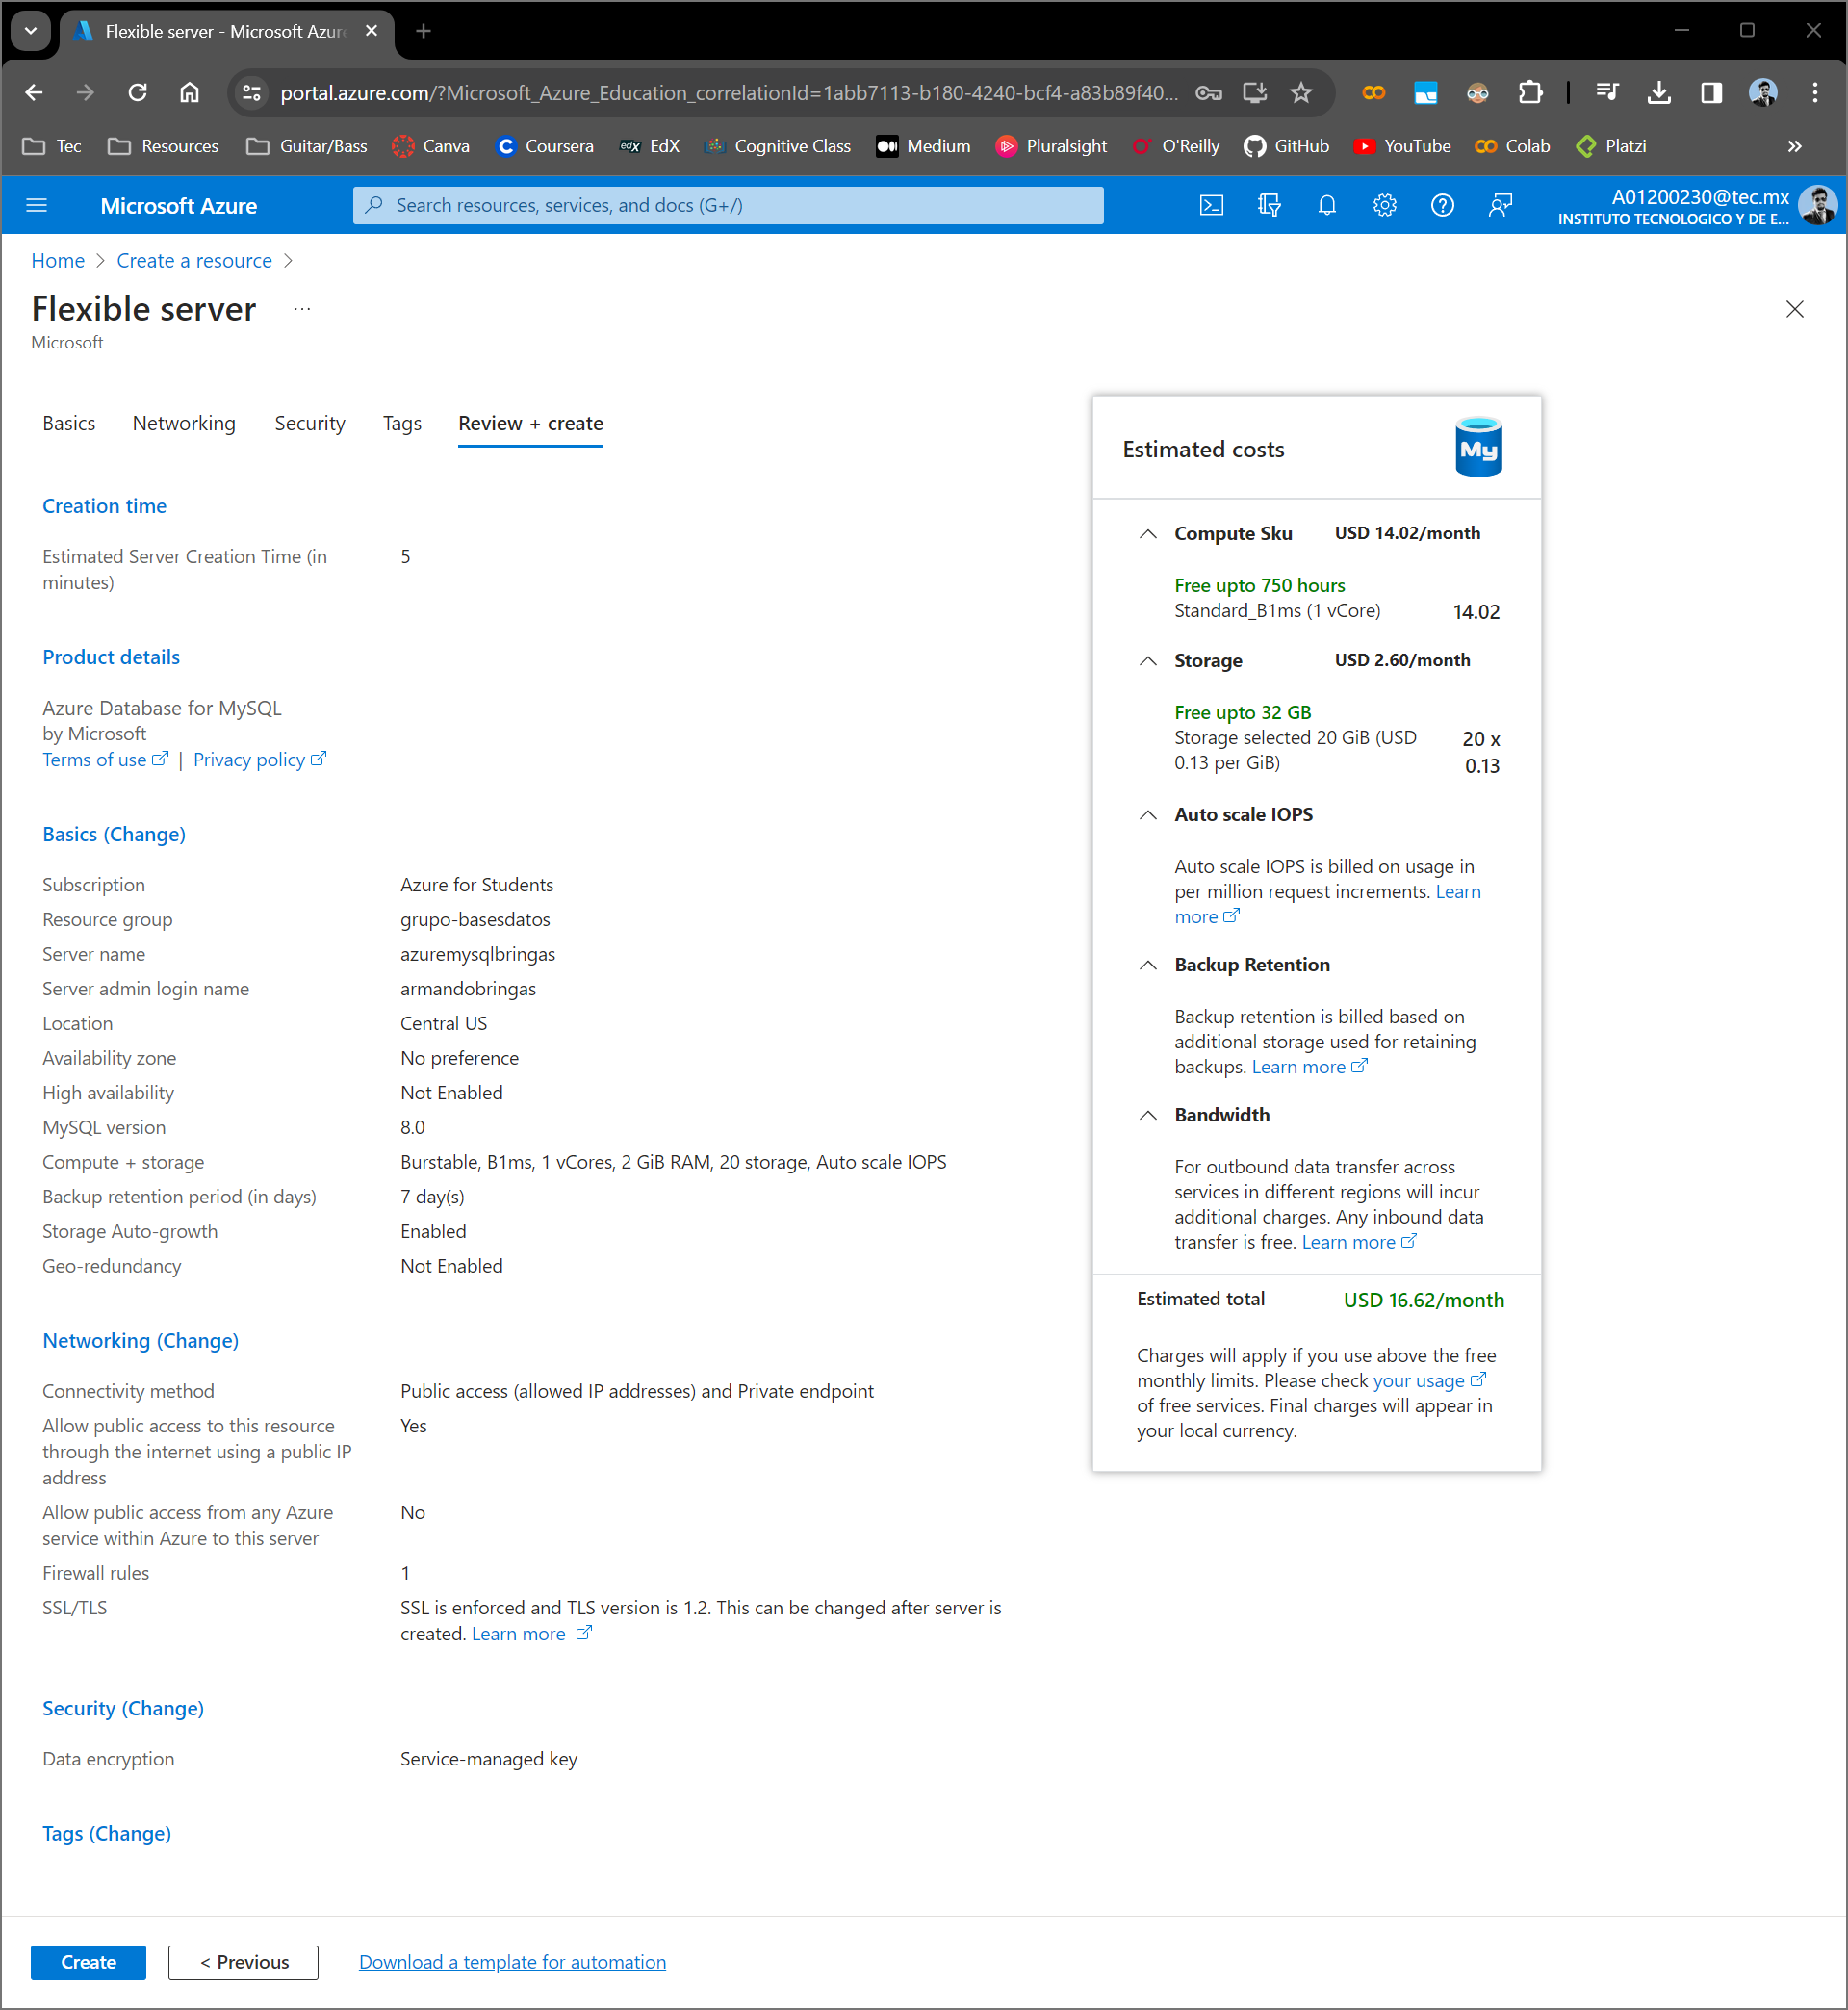
\includegraphics[width=.7\linewidth]{M4_Servicios_Cómputo_en_la_Nube/Tarea_6_Creación_sistema_administración_Base_de_Datos/reporte/figuras/1_1_1_Azure_DBMS.png}
    \captionof{lstlisting}{Creación del DBMS en Azure}
    \label{fig:1_1_1_Azure_DBMS}
\end{figure}

La creación del nuevo recurso tomó unos minutos, pero en la figura \ref{fig:1_1_2_Azure_DBMS} se observa que su creación fue completada.

\begin{figure}[H]
    \centering
    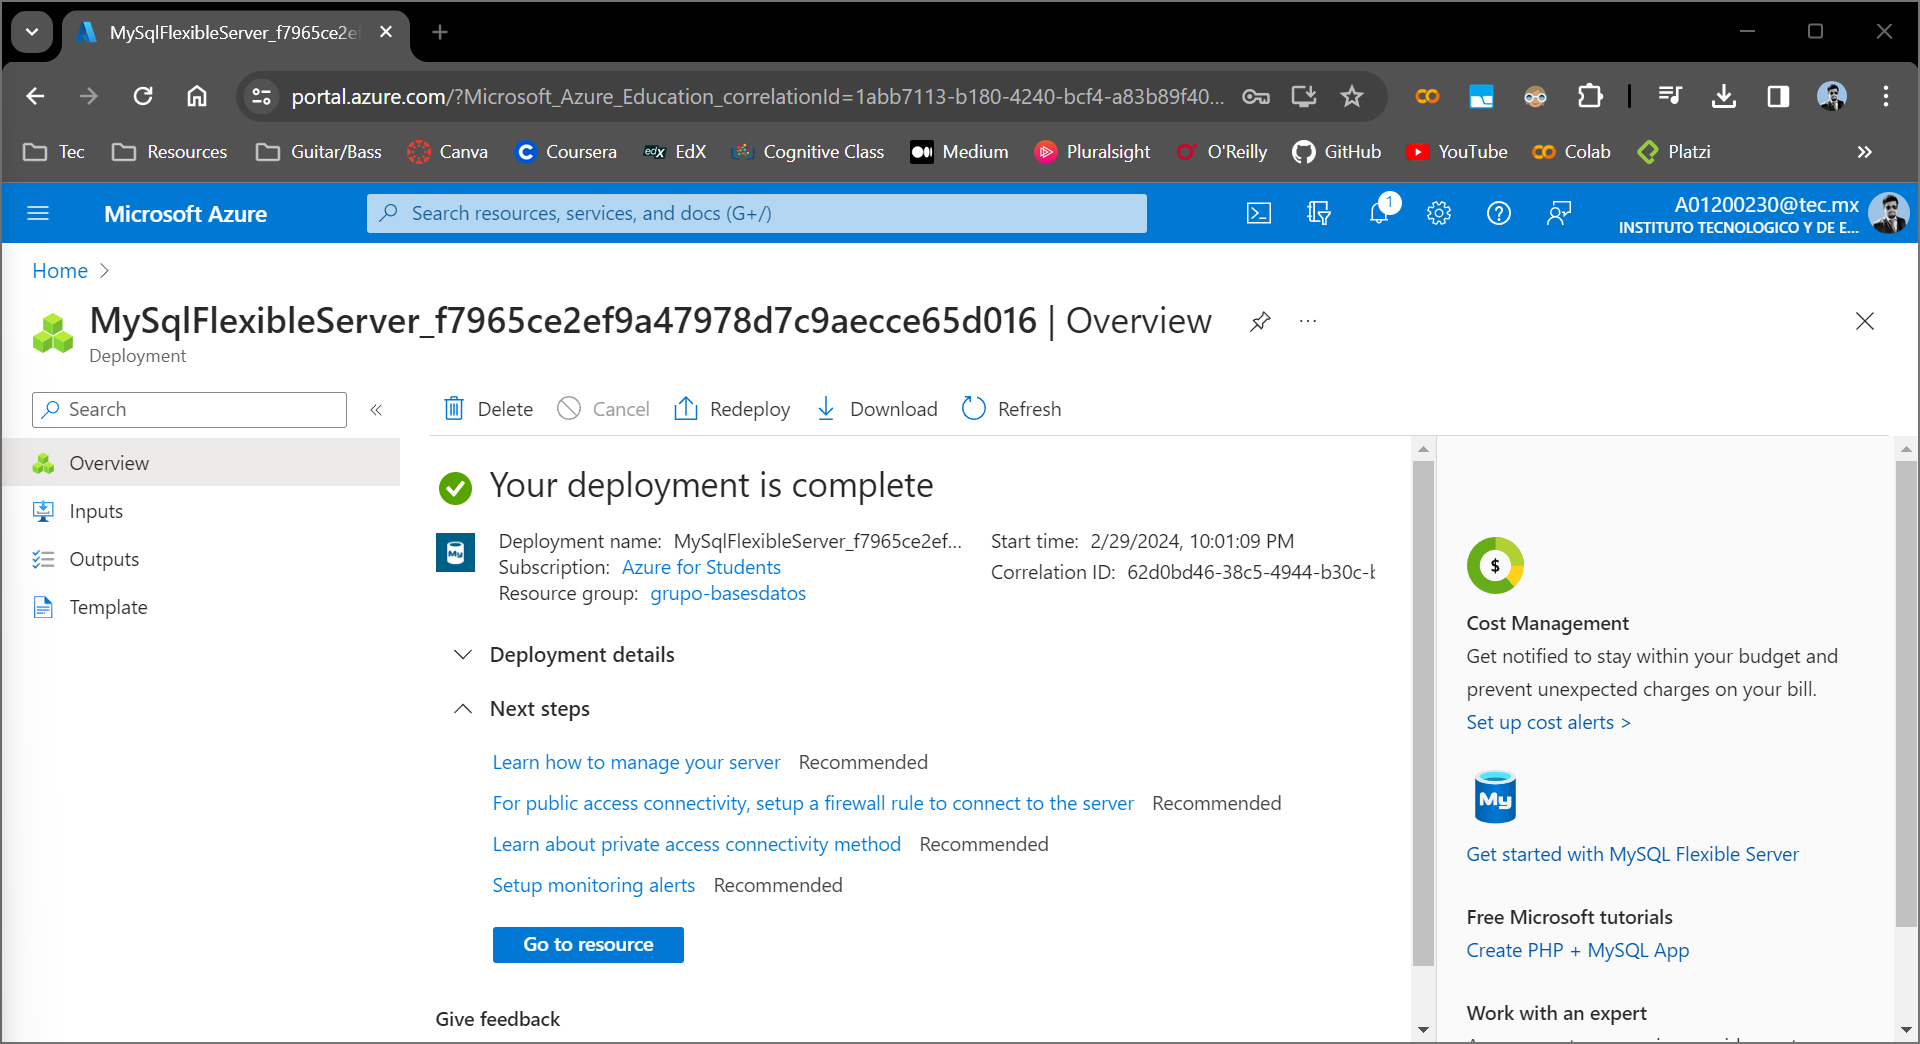
\includegraphics[width=.85\linewidth]{M4_Servicios_Cómputo_en_la_Nube/Tarea_6_Creación_sistema_administración_Base_de_Datos/reporte/figuras/1_1_2_Azure_DBMS.png}
    \captionof{lstlisting}{Creación del DBMS en Azure}
    \label{fig:1_1_2_Azure_DBMS}
\end{figure}

Al momento de ir al recurso observamos diferentes propiedades de las cuales obtenemos el nombre del servidor al cual accederemos a través de la siguiente URL pública:\\
\textbf{azuremysqlbringas.mysql.database.azure.com} como se puede ver en la figura \ref{fig:1_1_3_Azure_DBMS}.

\begin{figure}[H]
    \centering
    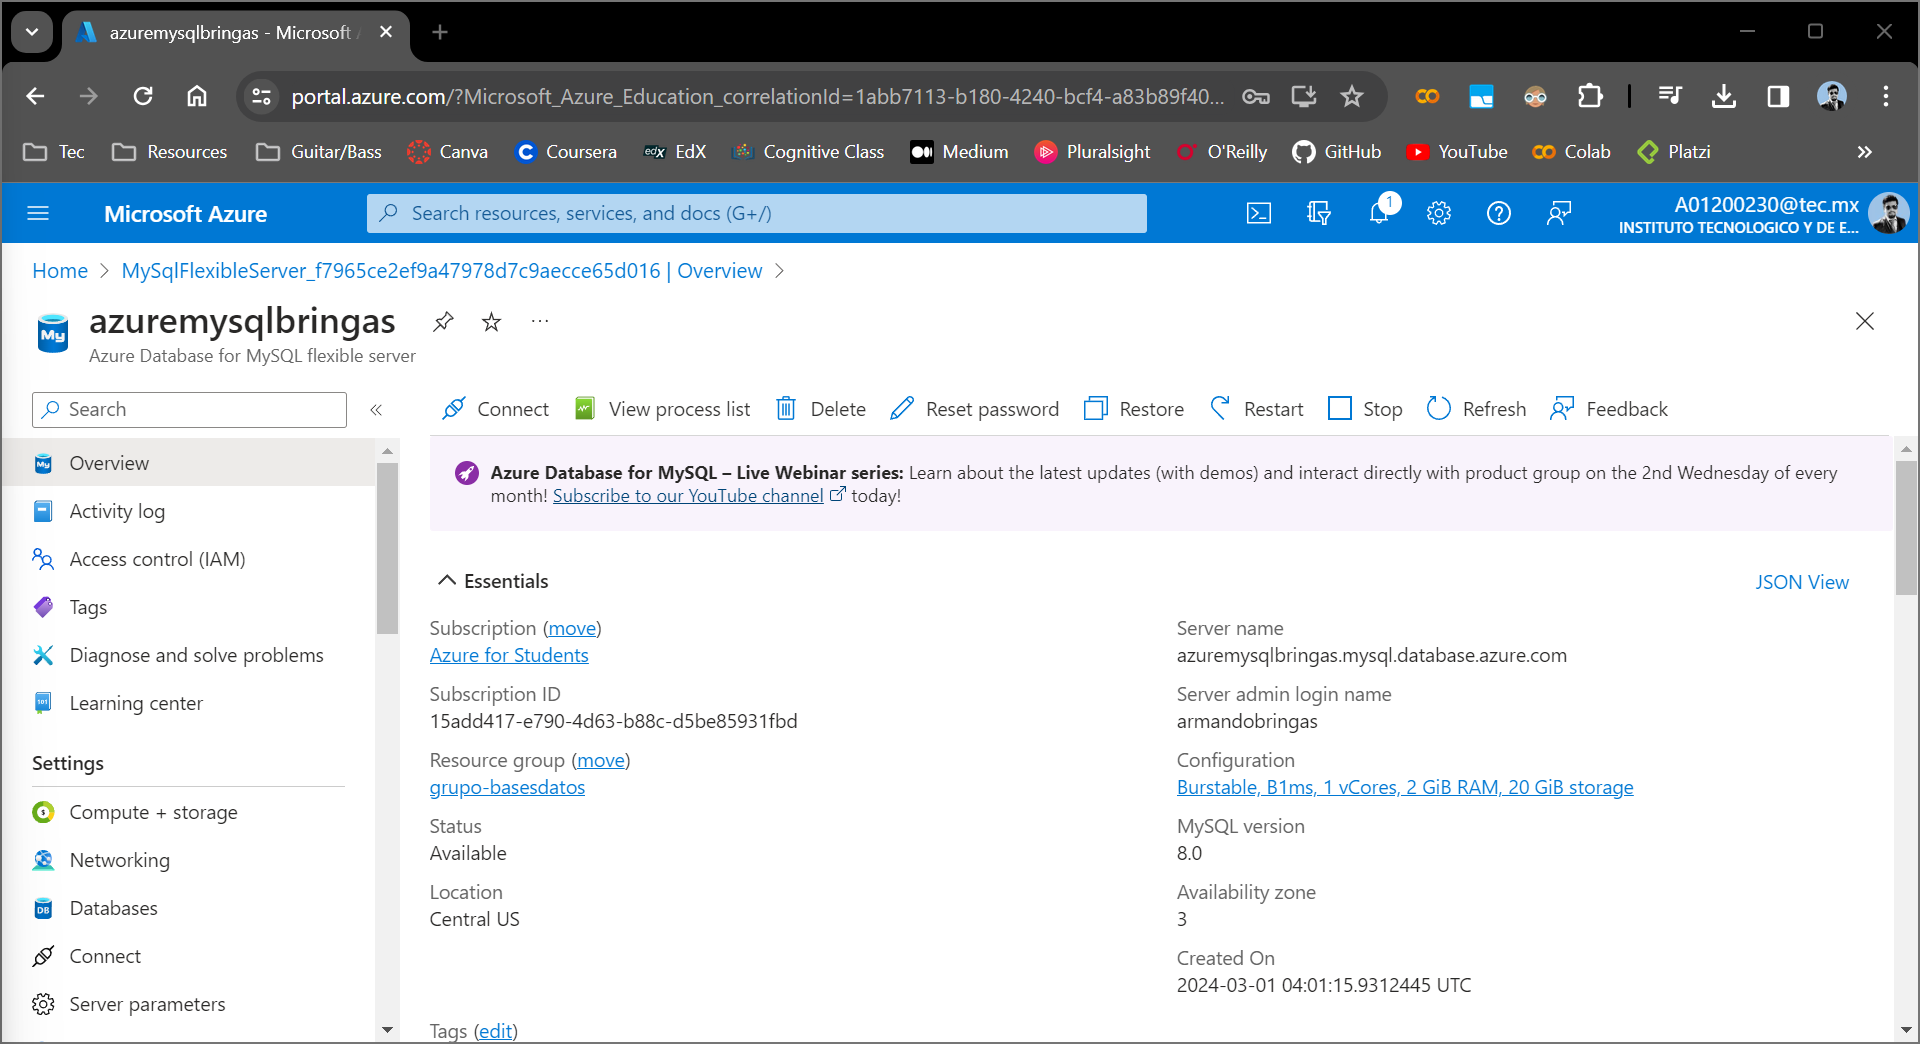
\includegraphics[width=.85\linewidth]{M4_Servicios_Cómputo_en_la_Nube/Tarea_6_Creación_sistema_administración_Base_de_Datos/reporte/figuras/1_1_3_Azure_DBMS.png}
    \captionof{lstlisting}{Creación del DBMS en Azure}
    \label{fig:1_1_3_Azure_DBMS}
\end{figure}

\vspace{10em}

\subsection{Creación de la base de datos}

Posteriormente en nuestro servidor creamos la base de datos con el nombre de \textbf{compradores} como se puede ver en la figura \ref{fig:1_2_1_Azure_DBMS}.

\begin{figure}[H]
    \centering
    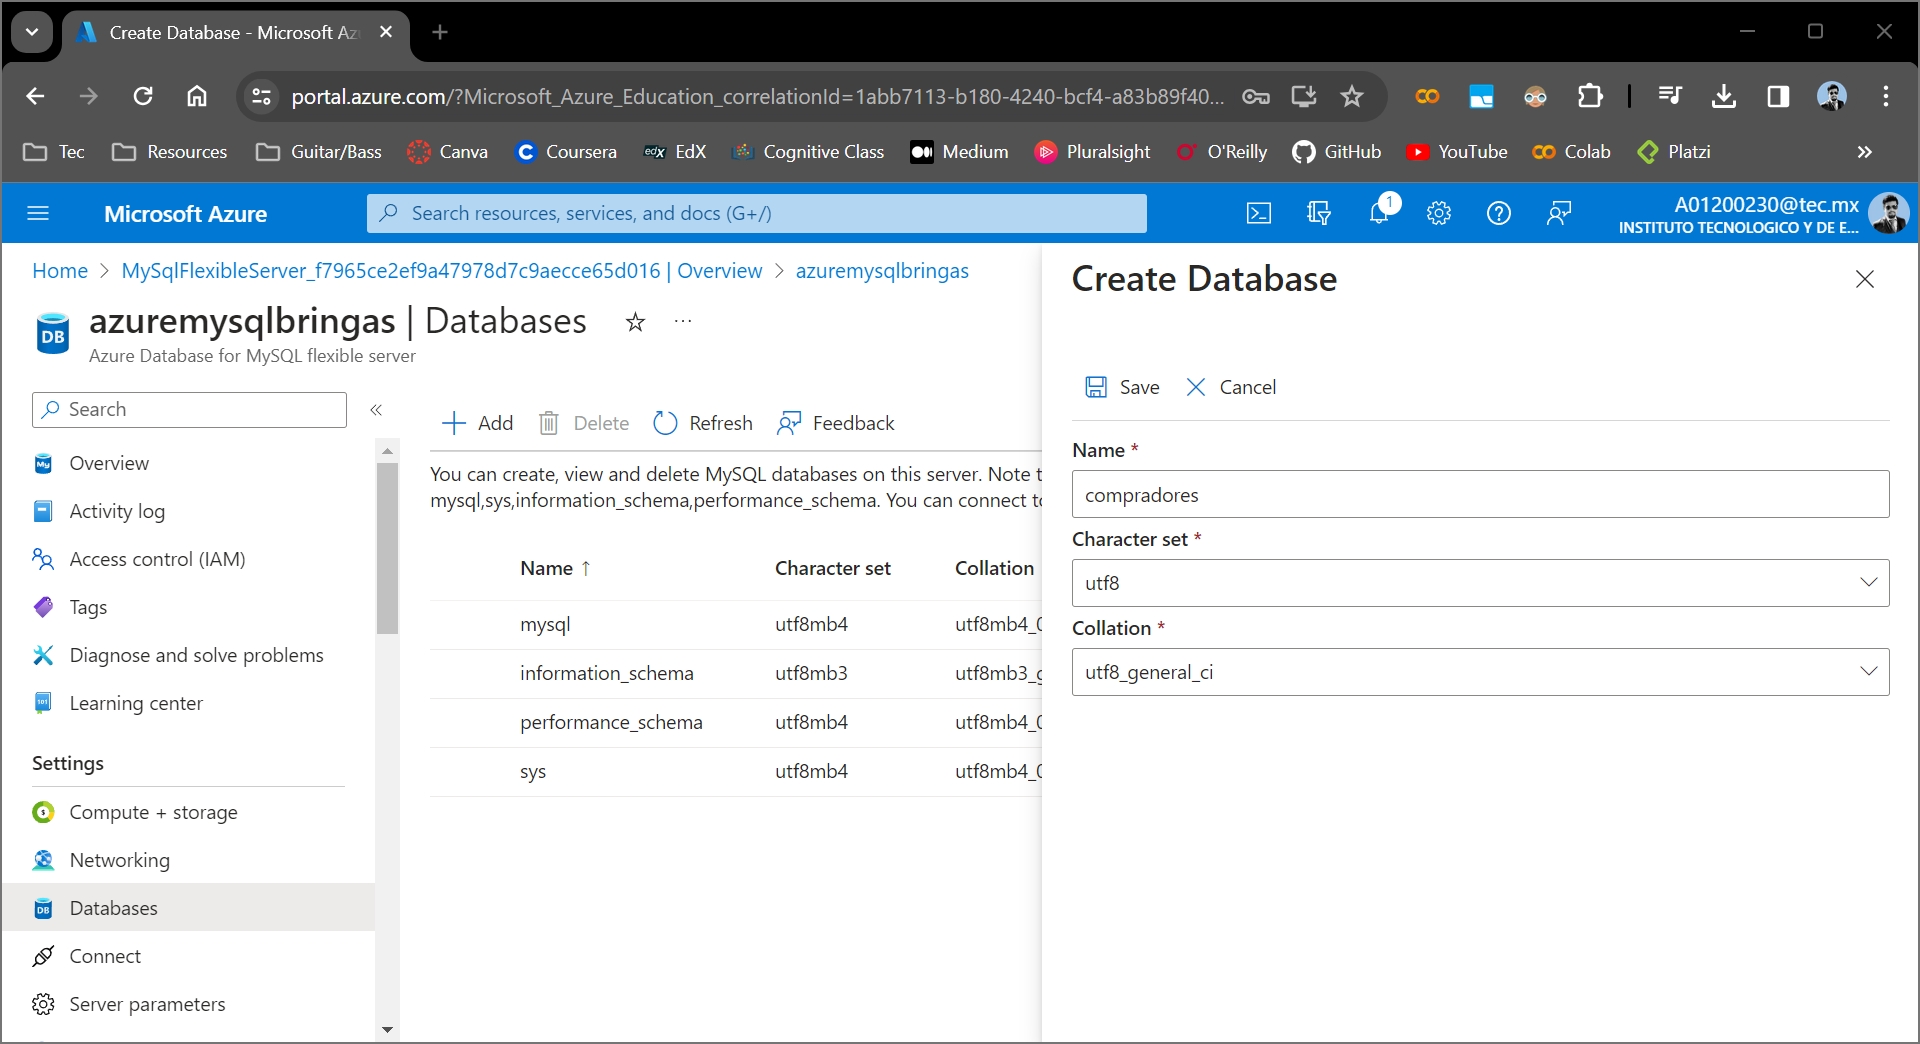
\includegraphics[width=.7\linewidth]{M4_Servicios_Cómputo_en_la_Nube/Tarea_6_Creación_sistema_administración_Base_de_Datos/reporte/figuras/1_2_1_Azure_DBMS.png}
    \captionof{lstlisting}{Creación de la base de datos en Azure}
    \label{fig:1_2_1_Azure_DBMS}
\end{figure}

El siguiente paso previo a la carga de registros nuevos en nuestra nueva base de datos es ingresar a la misma a través de la aplicación de \textbf{MySQL Workbench}, al momento de cargar los valores de configuración y de acceso de usuario con el que creamos nuestra base de datos en el portal de Azure probamos la conexción y vemos que esta fue exitosa como se muestra en la figura \ref{fig:1_2_2_Azure_DBMS}.

\begin{figure}[H]
    \centering
    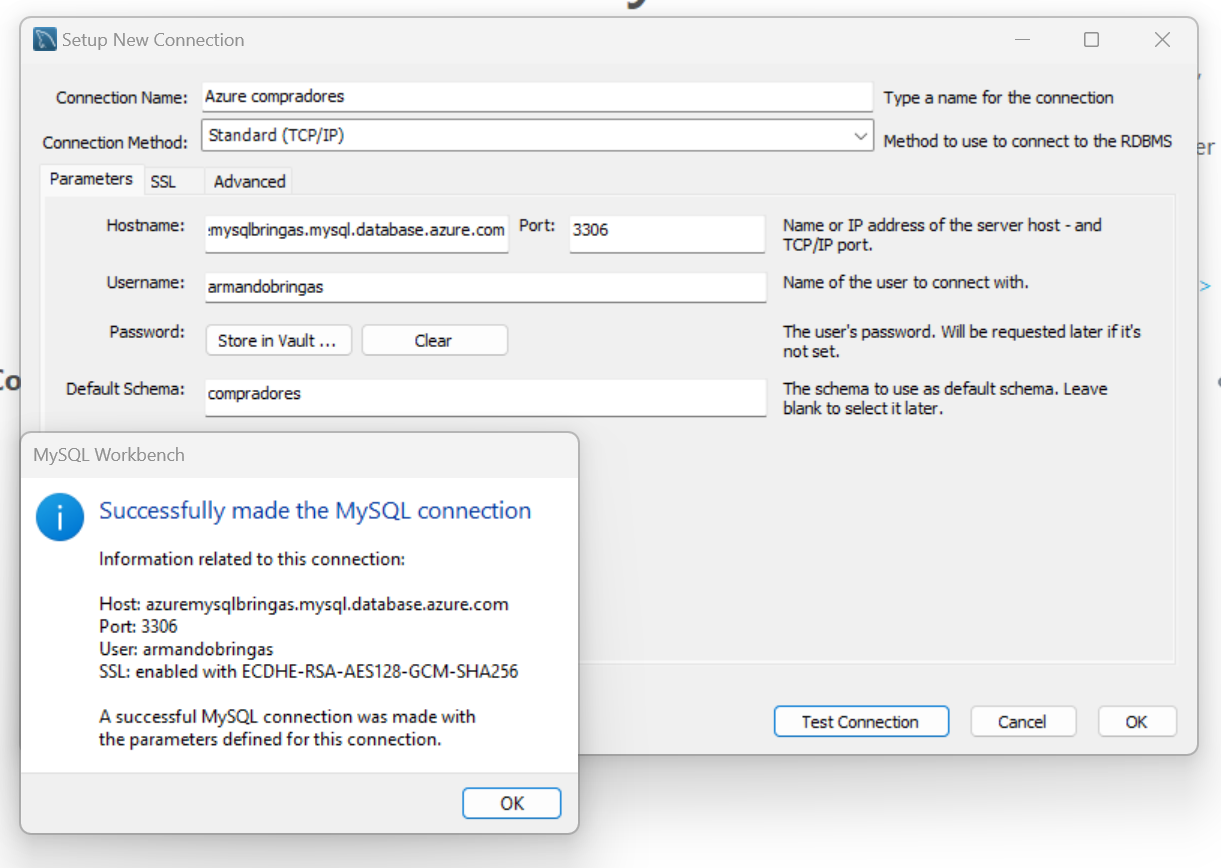
\includegraphics[width=.7\linewidth]{M4_Servicios_Cómputo_en_la_Nube/Tarea_6_Creación_sistema_administración_Base_de_Datos/reporte/figuras/1_2_2_Azure_DBMS.png}
    \captionof{lstlisting}{Estableciendo conexión don el DBMS de Azure}
    \label{fig:1_2_2_Azure_DBMS}
\end{figure}

\subsection{Carga de los registros nuevos}

En \textit{mySQL} accedemos a la nueva base datos que creamos a través de la opción de \textit{schemas} para poder ver la base de datos y sus componentes como tablas y vistas. Posteriormente creamos una tabla con una estructura como se ve en la figura \ref{fig:1_3_1_Azure_DBMS} para poder alojar la información la cual será una base de datos que representa la información ficticia de clientes compradores.

\begin{figure}[H]
    \centering
    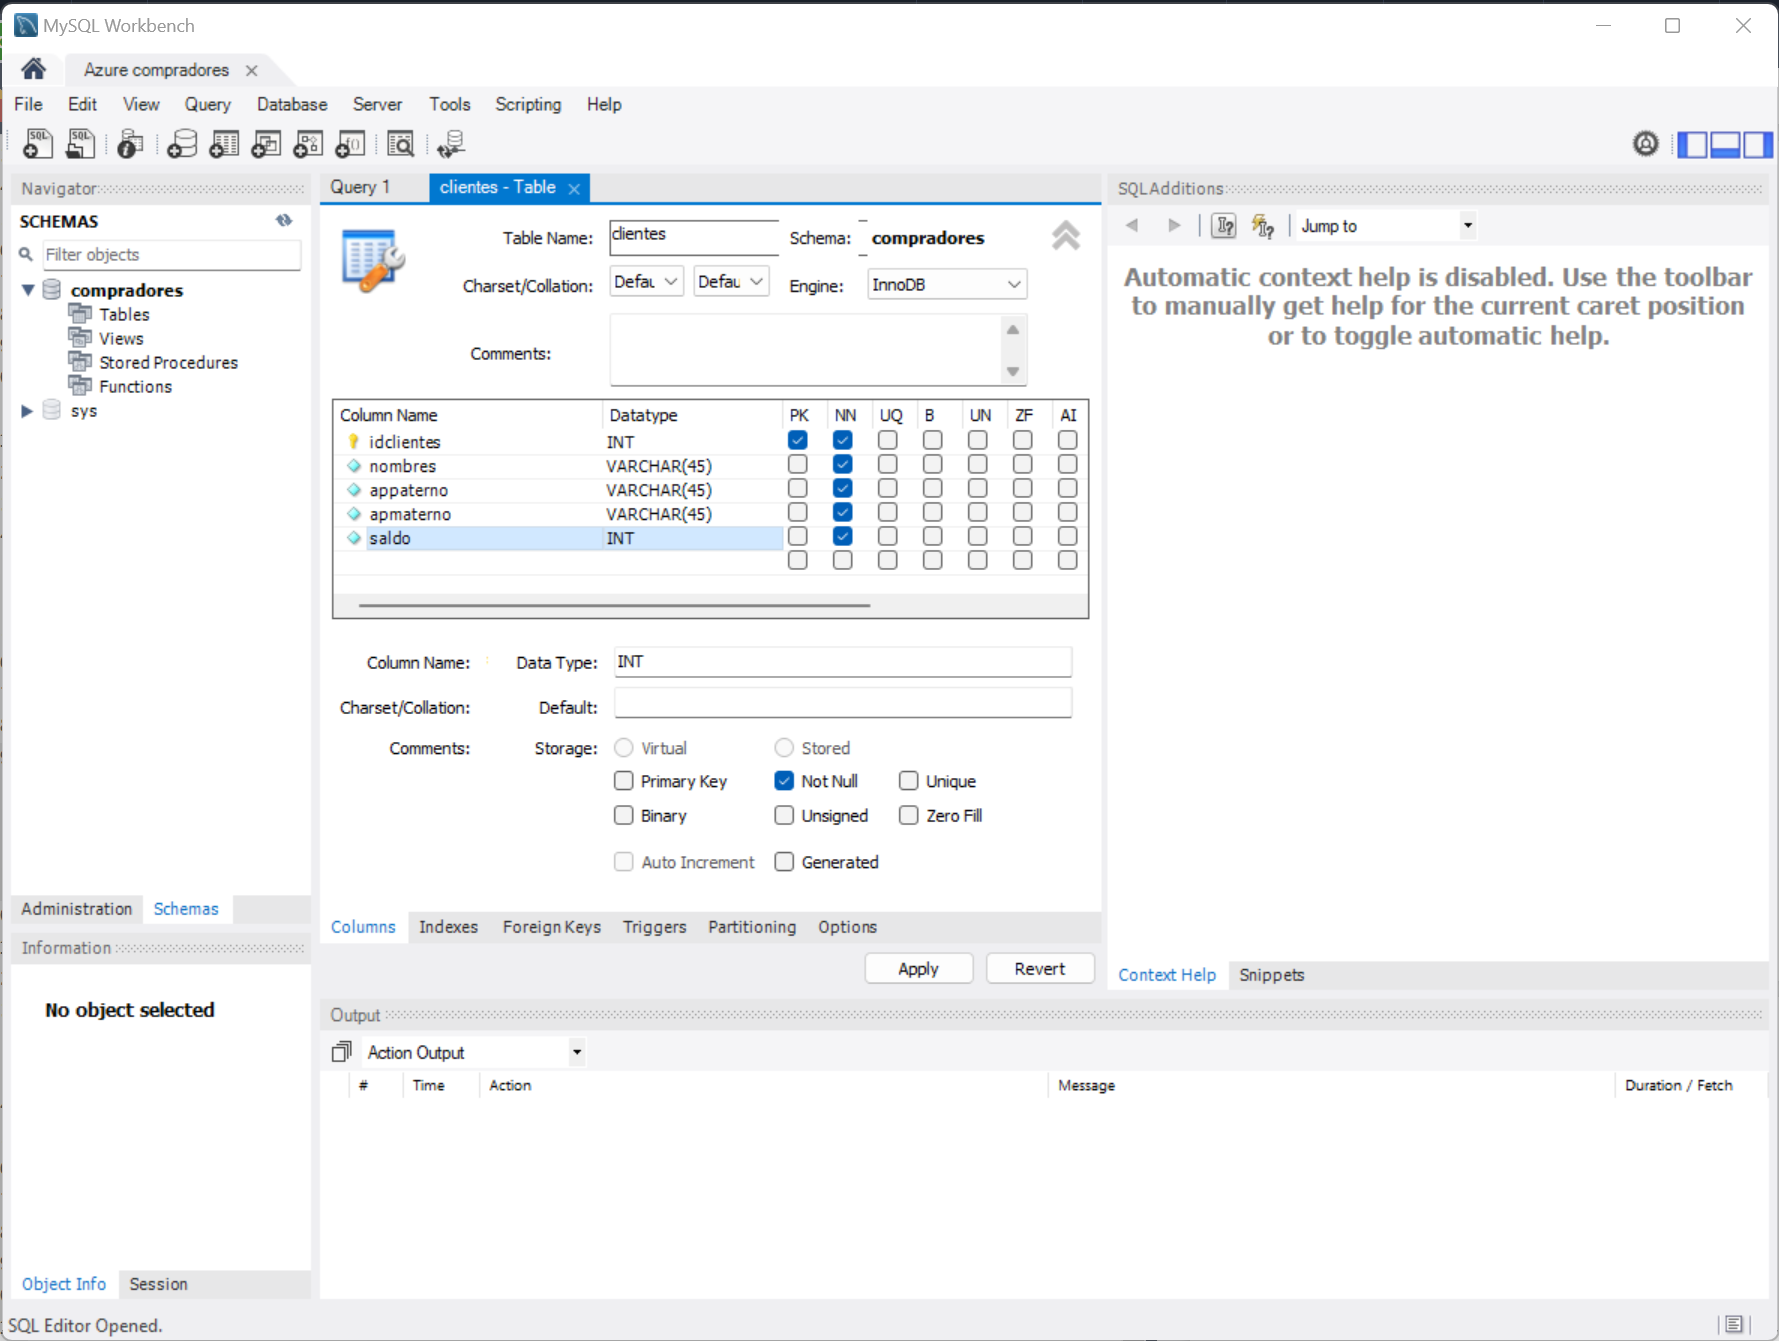
\includegraphics[width=.6\linewidth]{M4_Servicios_Cómputo_en_la_Nube/Tarea_6_Creación_sistema_administración_Base_de_Datos/reporte/figuras/1_3_1_Azure_DBMS.png}
    \captionof{lstlisting}{Carga de los nuevos registros de la Base de Datos de MySQL}
    \label{fig:1_3_1_Azure_DBMS}
\end{figure}


En la figura \ref{fig:1_3_2_Azure_DBMS} podemos observar las sentencias que SQL estará mandando a nuestro manejador de Base de Datos en la Nube.

\begin{figure}[H]
    \centering
    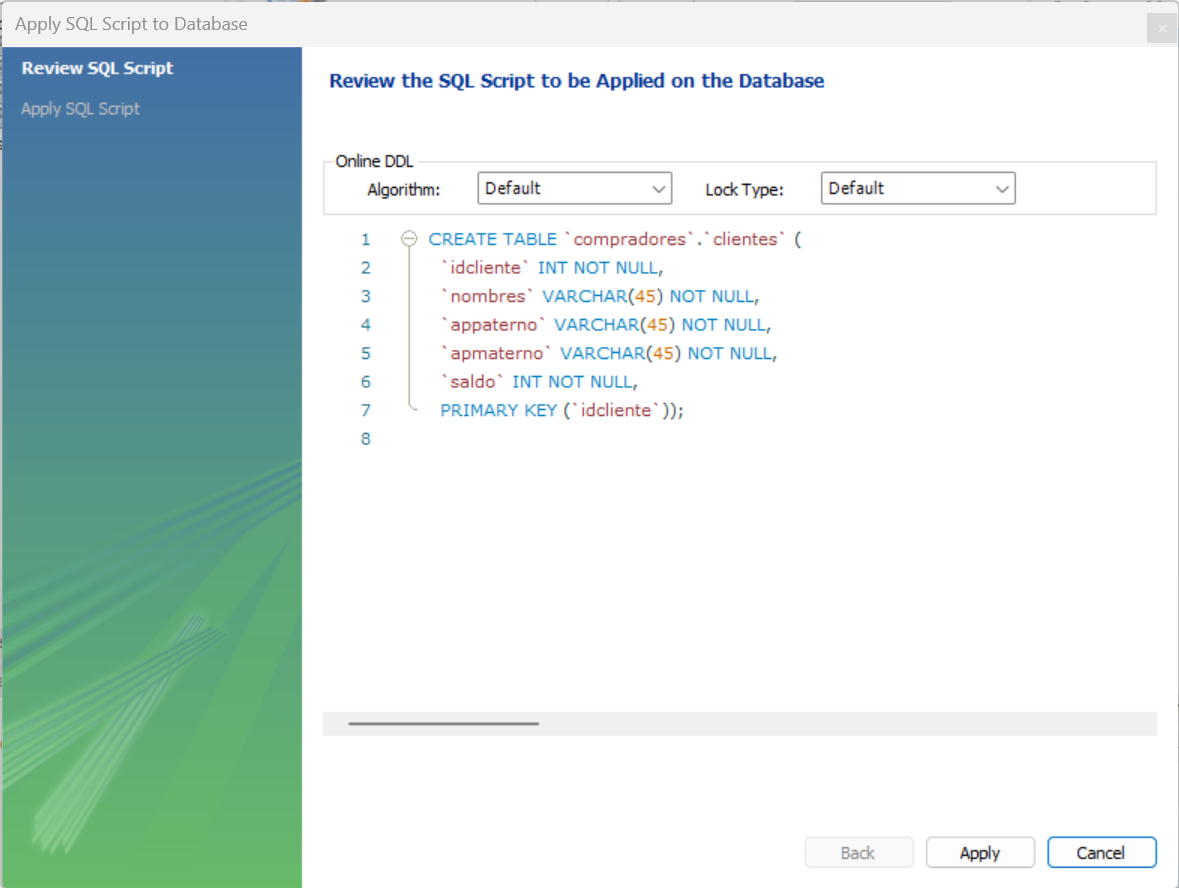
\includegraphics[width=.6\linewidth]{M4_Servicios_Cómputo_en_la_Nube/Tarea_6_Creación_sistema_administración_Base_de_Datos/reporte/figuras/1_3_2_Azure_DBMS.png}
    \captionof{lstlisting}{Carga de los nuevos registros de la Base de Datos de MySQL}
    \label{fig:1_3_2_Azure_DBMS}
\end{figure}

Finalmente, populamos la tabla de clientes con algunos valores ficticios y al momento de mandar los datos a la nube observamos como los datos ingresados tienen un \textbf{id} el cual es asignado por el manejador como se observa en la figura \ref{fig:1_3_3_Azure_DBMS}, de esta manera podemos corroborar que los datos ya se encuentran en la nube.

\begin{figure}[H]
    \centering
    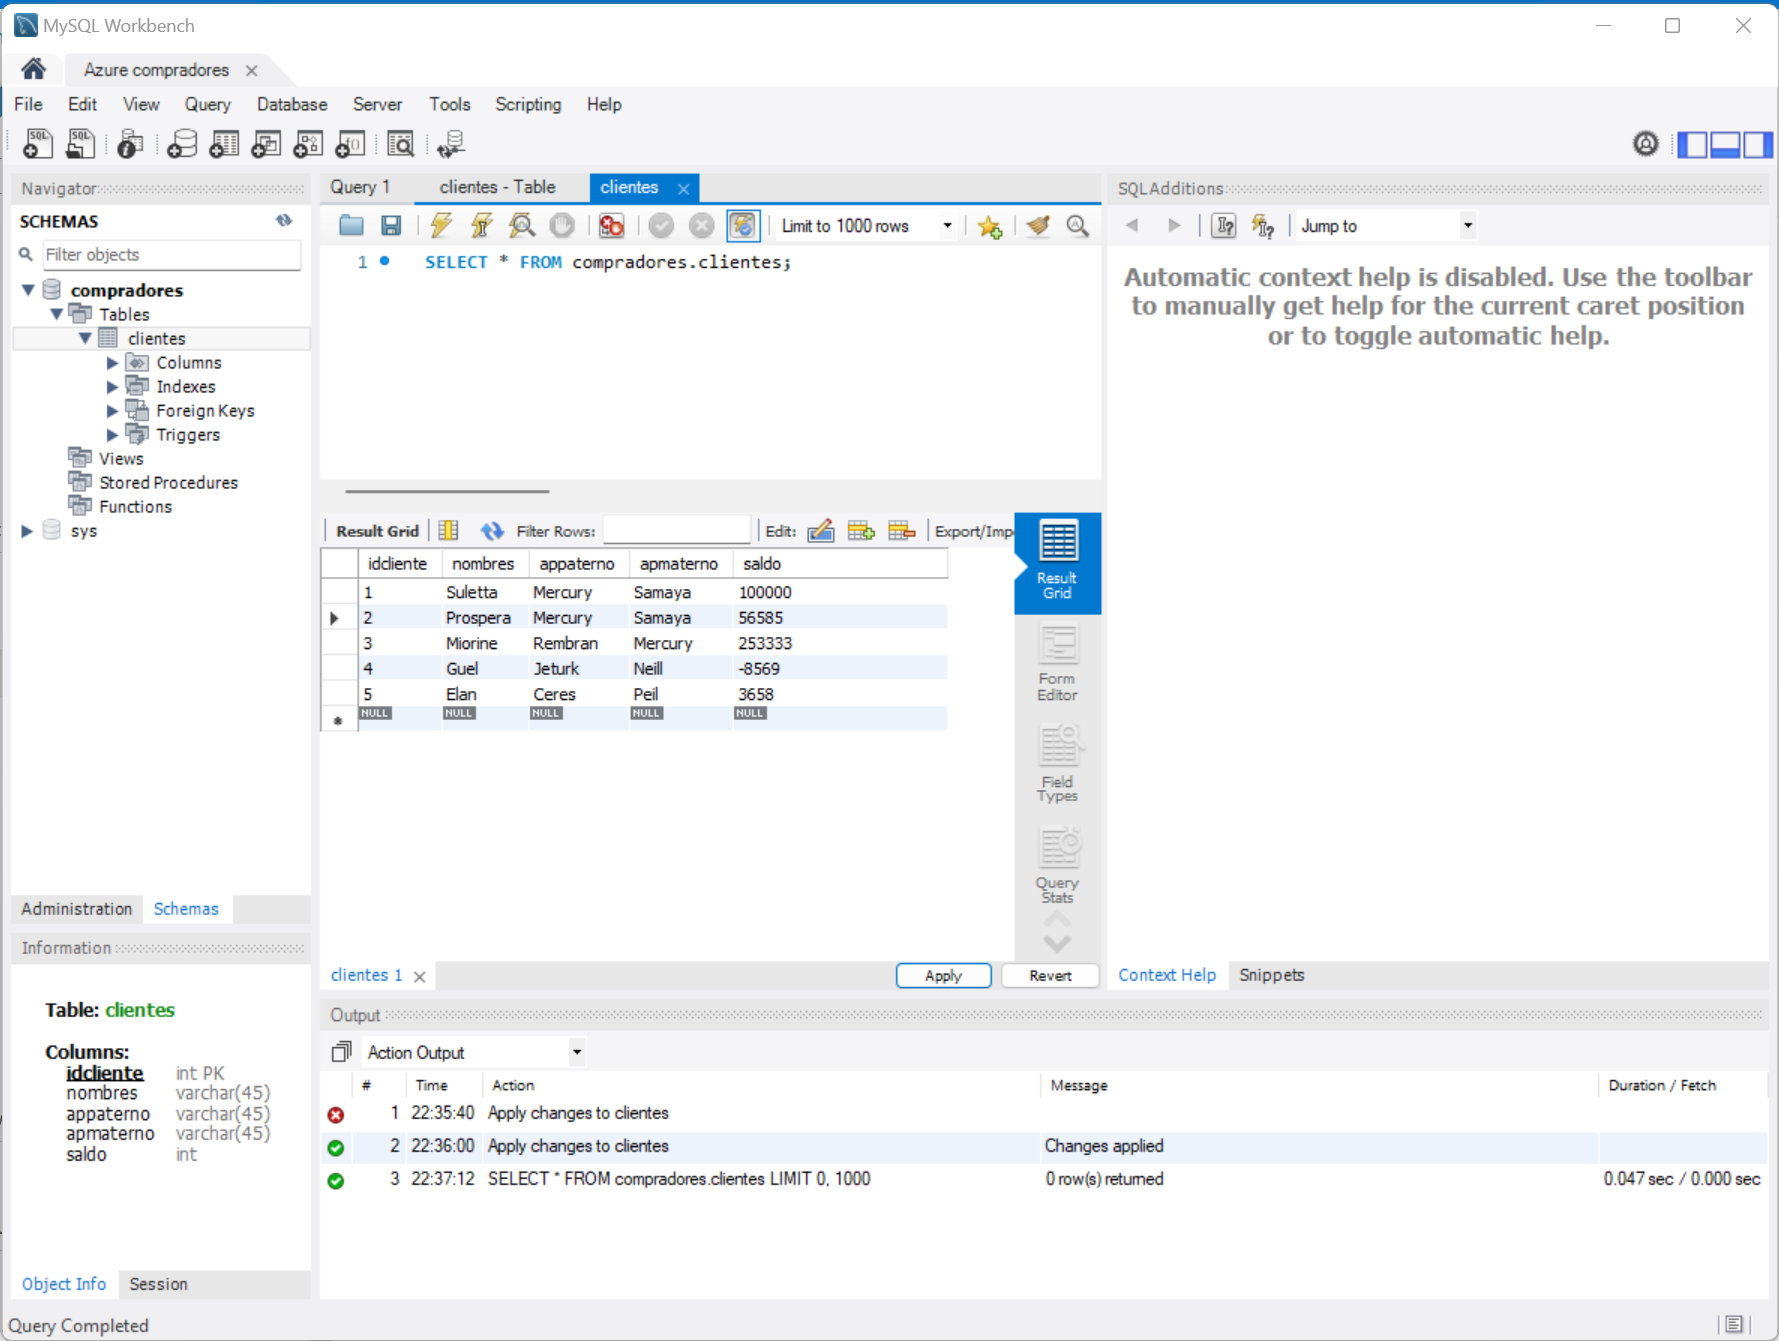
\includegraphics[width=1\linewidth]{M4_Servicios_Cómputo_en_la_Nube/Tarea_6_Creación_sistema_administración_Base_de_Datos/reporte/figuras/1_3_3_Azure_DBMS.png}
    \captionof{lstlisting}{Carga de los nuevos registros de la Base de Datos de MySQL}
    \label{fig:1_3_3_Azure_DBMS}
\end{figure}

\vspace{10em}

\section{DataBase Management System (DBMS) Google}

\subsection{Creación del DBMS en Google}

Para la creación del manejador de Base de Datos en Google Cloud procedemos a hacerlo a través de la plataforma de estudiantes de \textbf{Cloud Skills Boost} el cual tiene la desventaja de que tendrá una duración temporal con expiración del tiempo que dure el laboratorio al que ingresemos para realizar la actividad.

\begin{figure}[H]
    \centering
    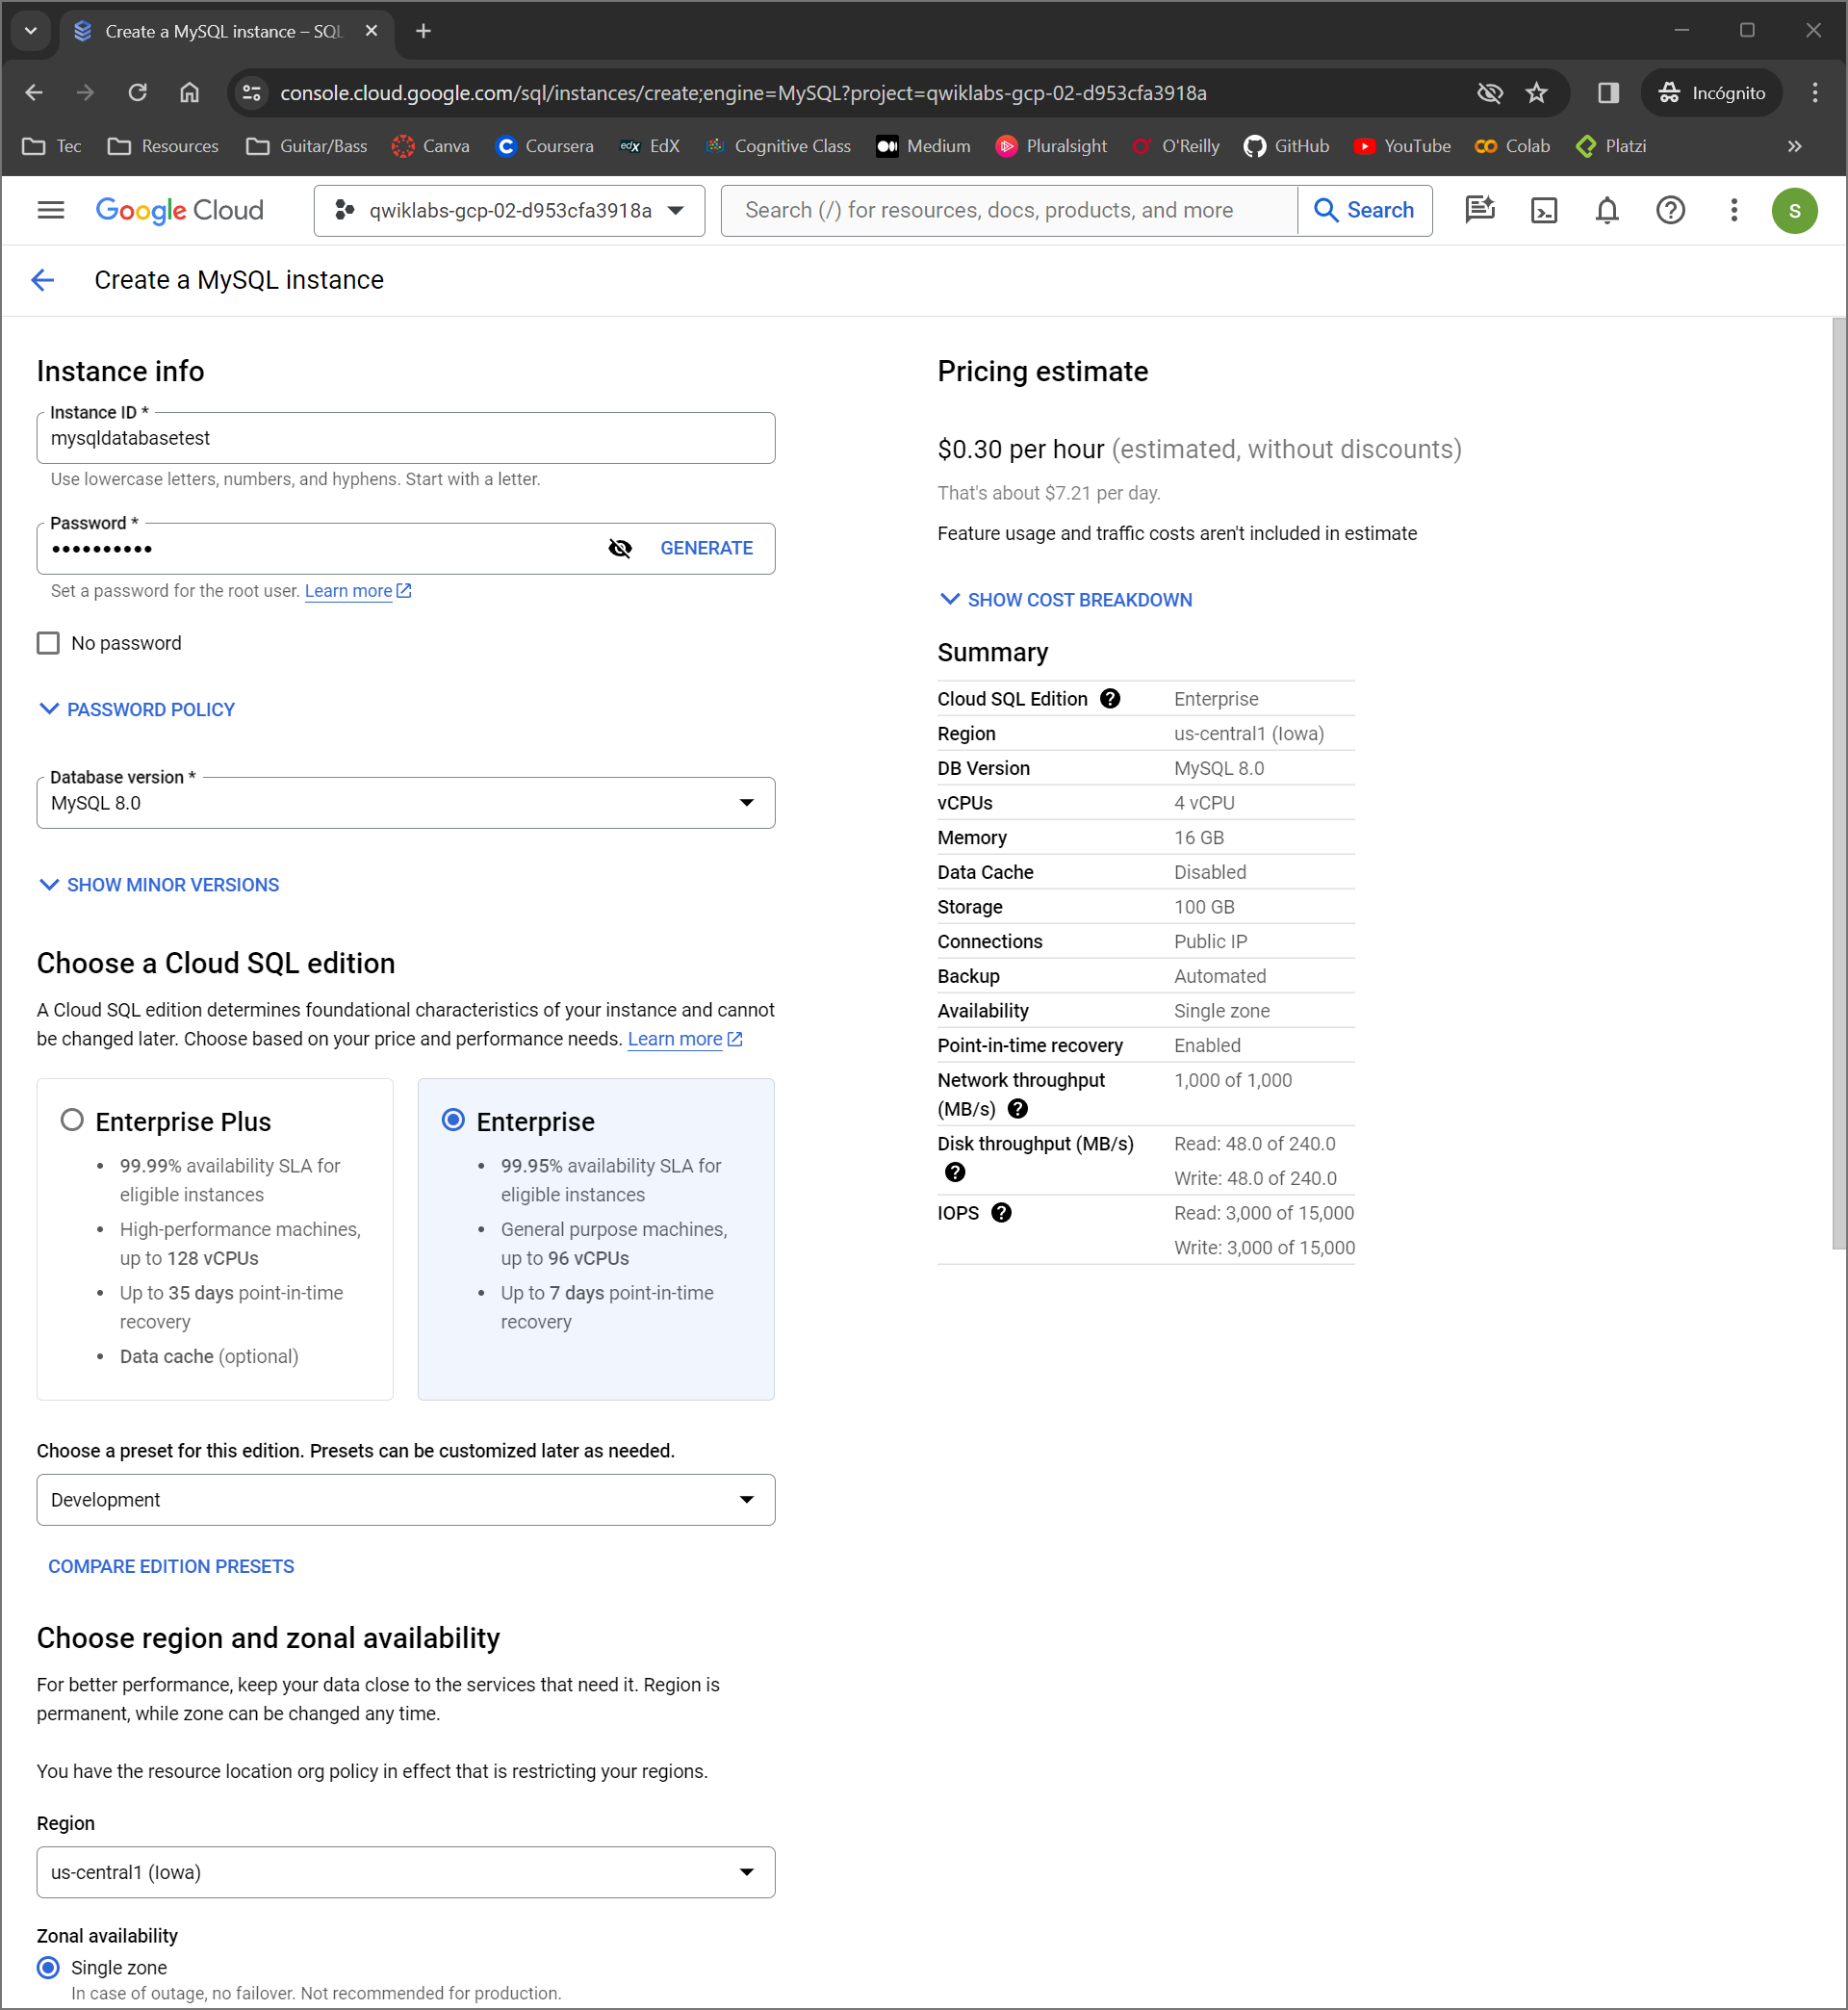
\includegraphics[width=.8\linewidth]{M4_Servicios_Cómputo_en_la_Nube/Tarea_6_Creación_sistema_administración_Base_de_Datos/reporte/figuras/2_1_1_Google_DBMS.png}
    \captionof{lstlisting}{Creación del DBMS en Google}
    \label{fig:2_1_1_Google_DBMS}
\end{figure}

Como podemos observar en la figura \ref{fig:2_1_1_Google_DBMS} se observa parte del proceso para la creación de la nueva instancia de nuestro manejador de bases de datos MySQL donde establecimos los siguientes parámetros:

\begin{itemize}
    \item \textbf{Instance ID}: Identificador de la instancia del manejador de bases de datos, en este caso lo identificamos como \textbf{mysqldatabasetest}.
    \item \textbf{Choose a configuration to star with}: En este caso seleccionamos la opción de \textbf{Development} ya que buscamos tener un entorno con buen desempeño pero no nos interesa que tenga alta disponibilidad.
    \item \textbf{Zonal availability}: \textbf{Single Zone} donde la instancia existe en una sola zona.
    \item \textbf{Instance IP assignment}: Se seleccionó la opción de \textbf{Public IP} para que el servidor de la base de datos este disponible.
\end{itemize}

En la siguiente figura \ref{fig:2_1_2_Google_DBMS}, podemos observar la creación del manejador de la base de datos de Google en la nube al cual accederemos con la siguiente dirección IP \textbf{34.31.124.77}.

\begin{figure}[H]
    \centering
    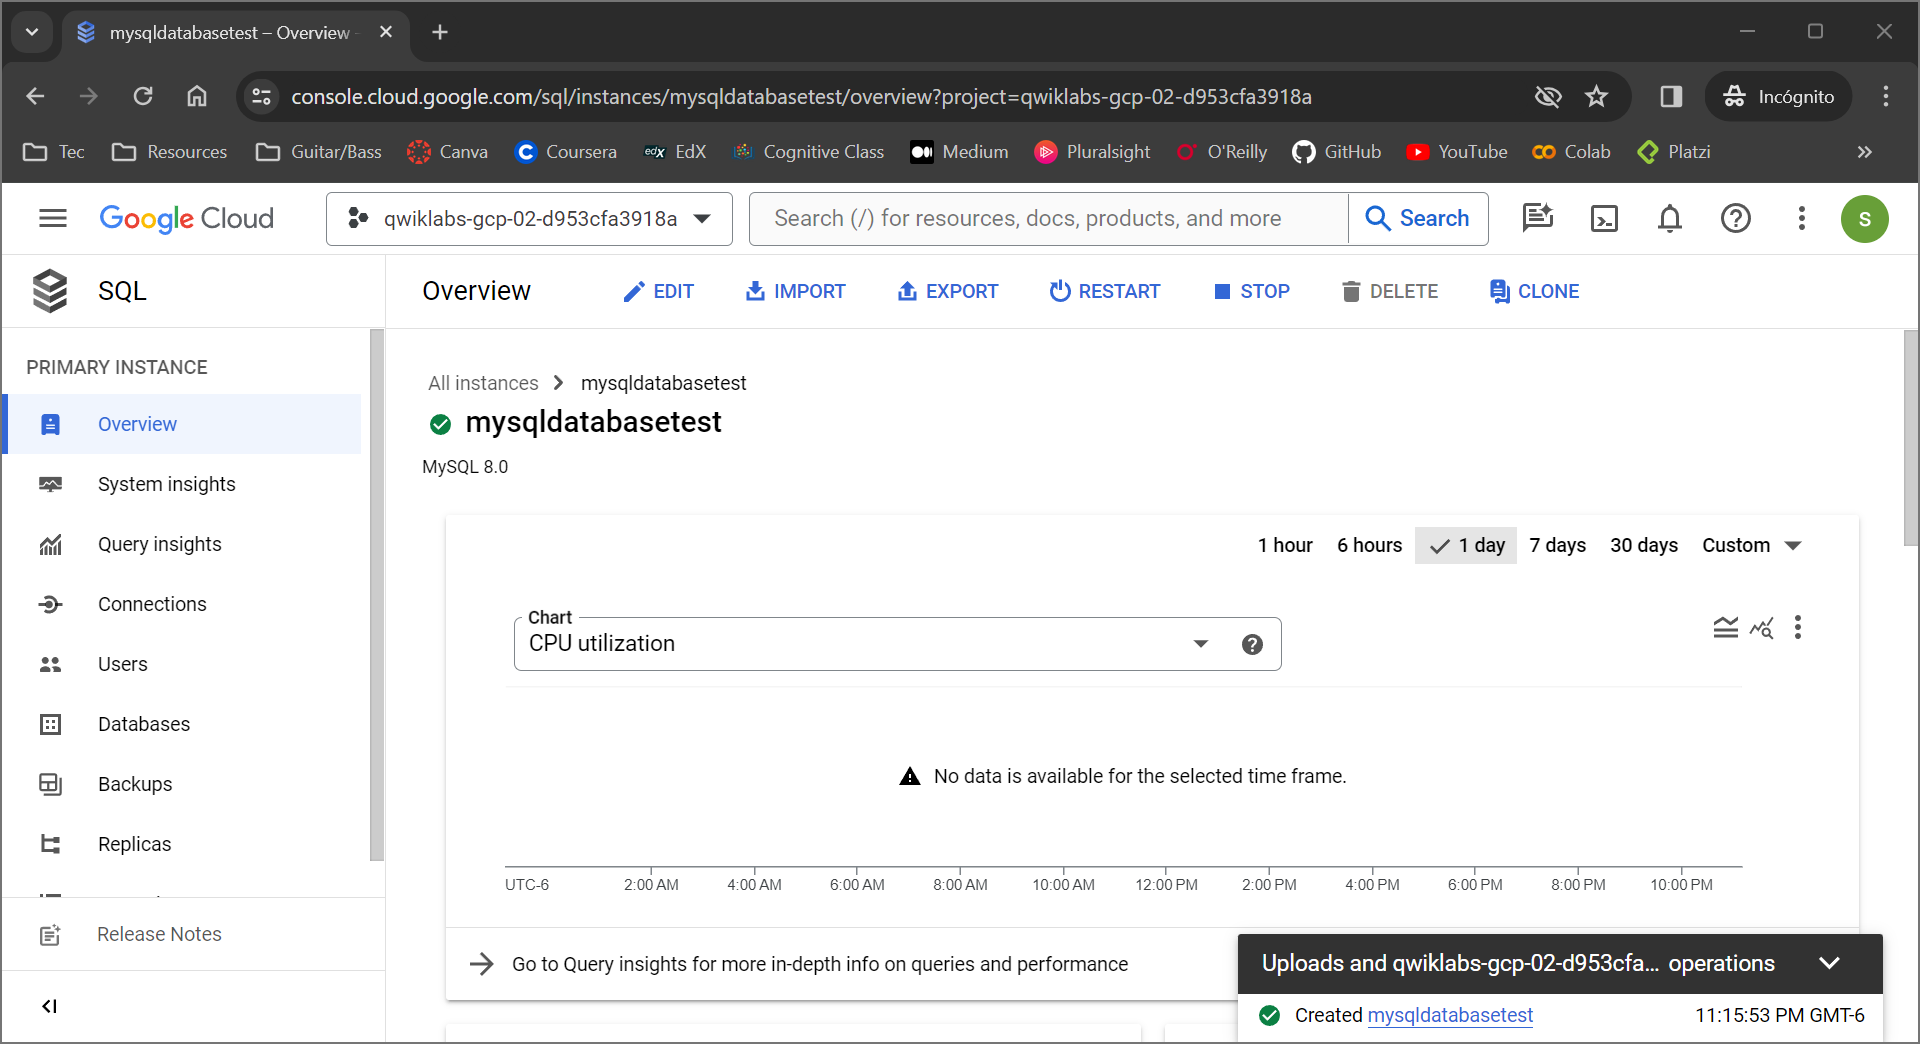
\includegraphics[width=.8\linewidth]{M4_Servicios_Cómputo_en_la_Nube/Tarea_6_Creación_sistema_administración_Base_de_Datos/reporte/figuras/2_1_2_Google_DBMS.png}
    \captionof{lstlisting}{Creación del DBMS en Google}
    \label{fig:2_1_2_Google_DBMS}
\end{figure}

\vspace{10em}

\subsection{Creación de la base de datos}

Previamente a la creación de nuestra base de datos, como se observa en la figura \ref{fig:2_2_1_Google_DBMS} establecemos el siguiente valor de red \textbf{0.0.0.0/0} para permitir cualquier conexión.

\begin{figure}[H]
    \centering
    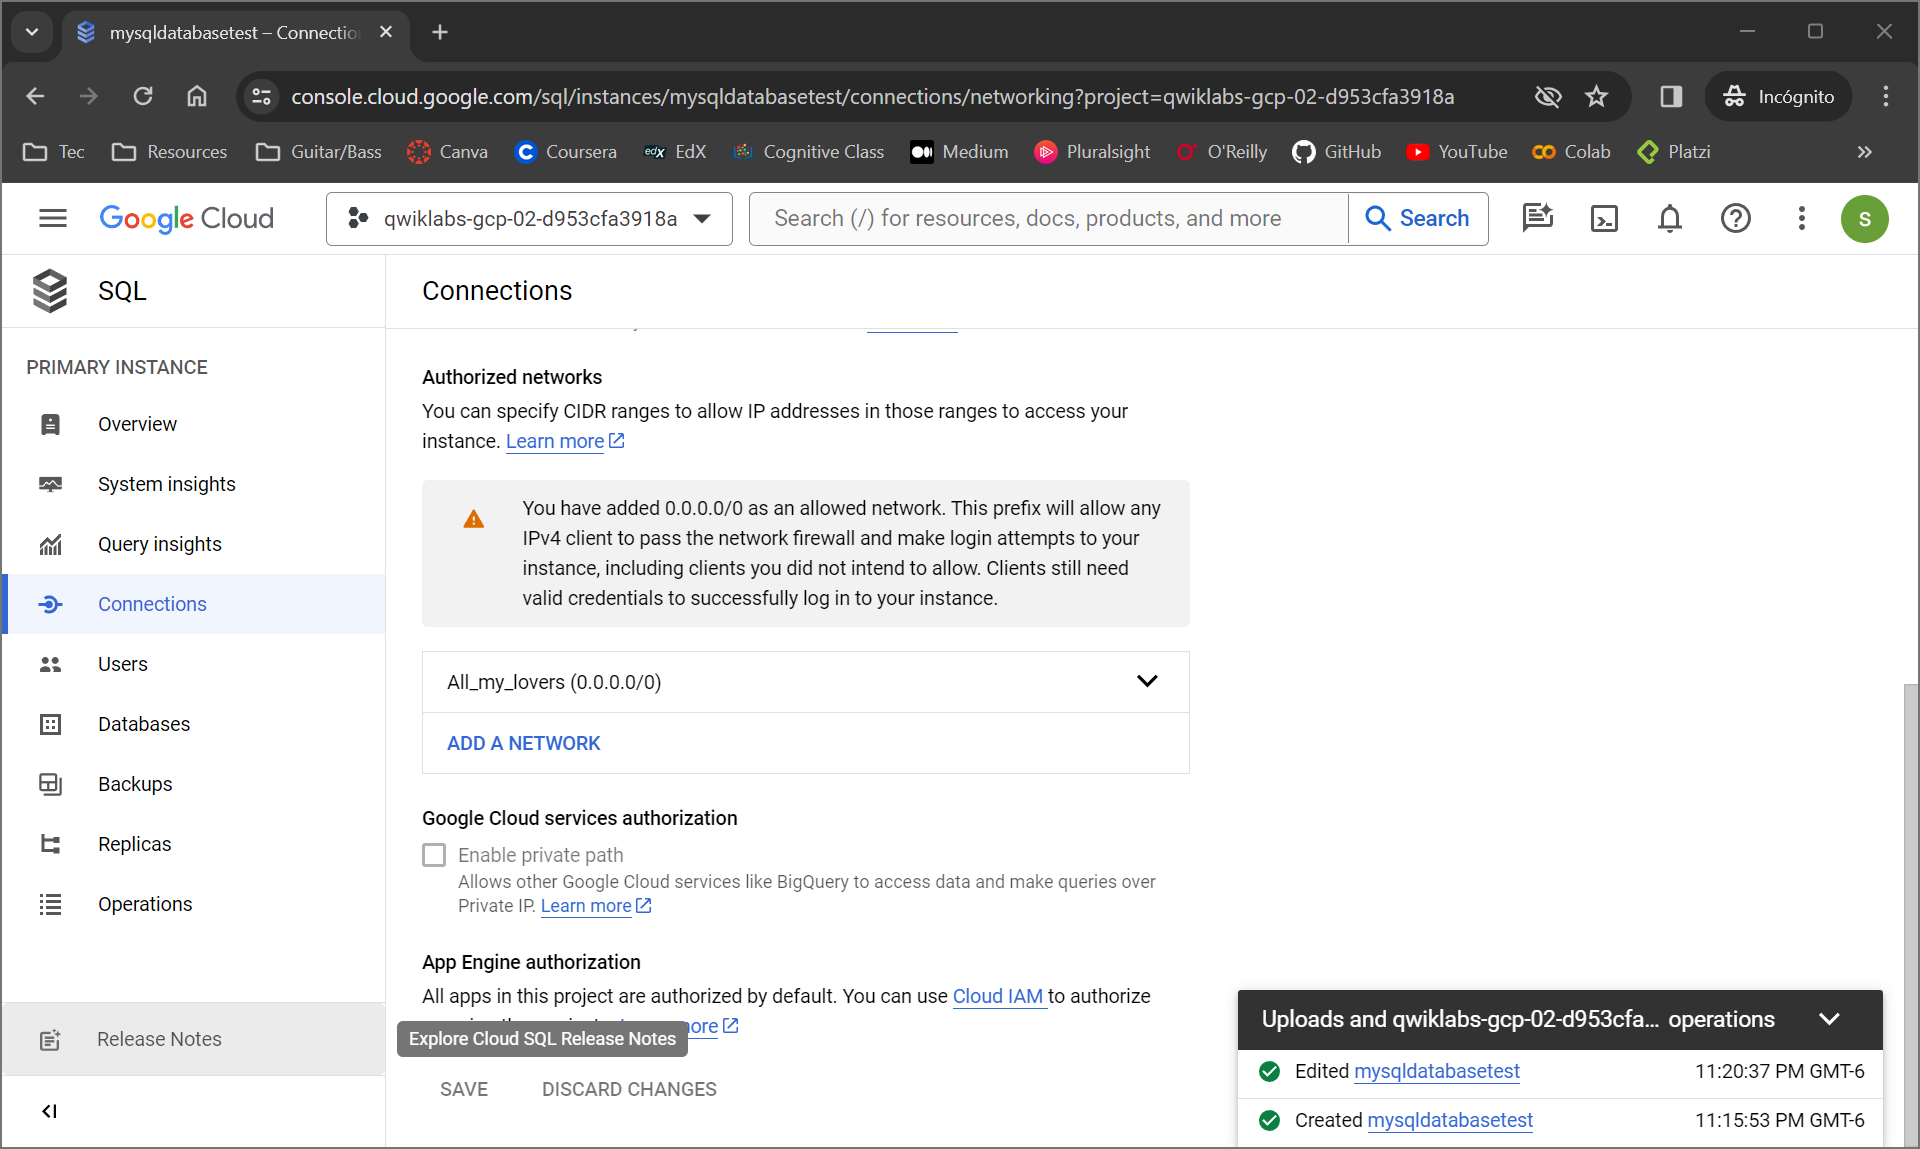
\includegraphics[width=.7\linewidth]{M4_Servicios_Cómputo_en_la_Nube/Tarea_6_Creación_sistema_administración_Base_de_Datos/reporte/figuras/2_2_1_Google_DBMS.png}
    \captionof{lstlisting}{Permitiendo conexiones externas en nuestro DBMS de Google}
    \label{fig:2_2_1_Google_DBMS}
\end{figure}

En la siguiente figura \ref{fig:2_2_2_Google_DBMS}, podemos observar la creación de la base de datos mySQL dentro de nuestro manejador.

\begin{figure}[H]
    \centering
    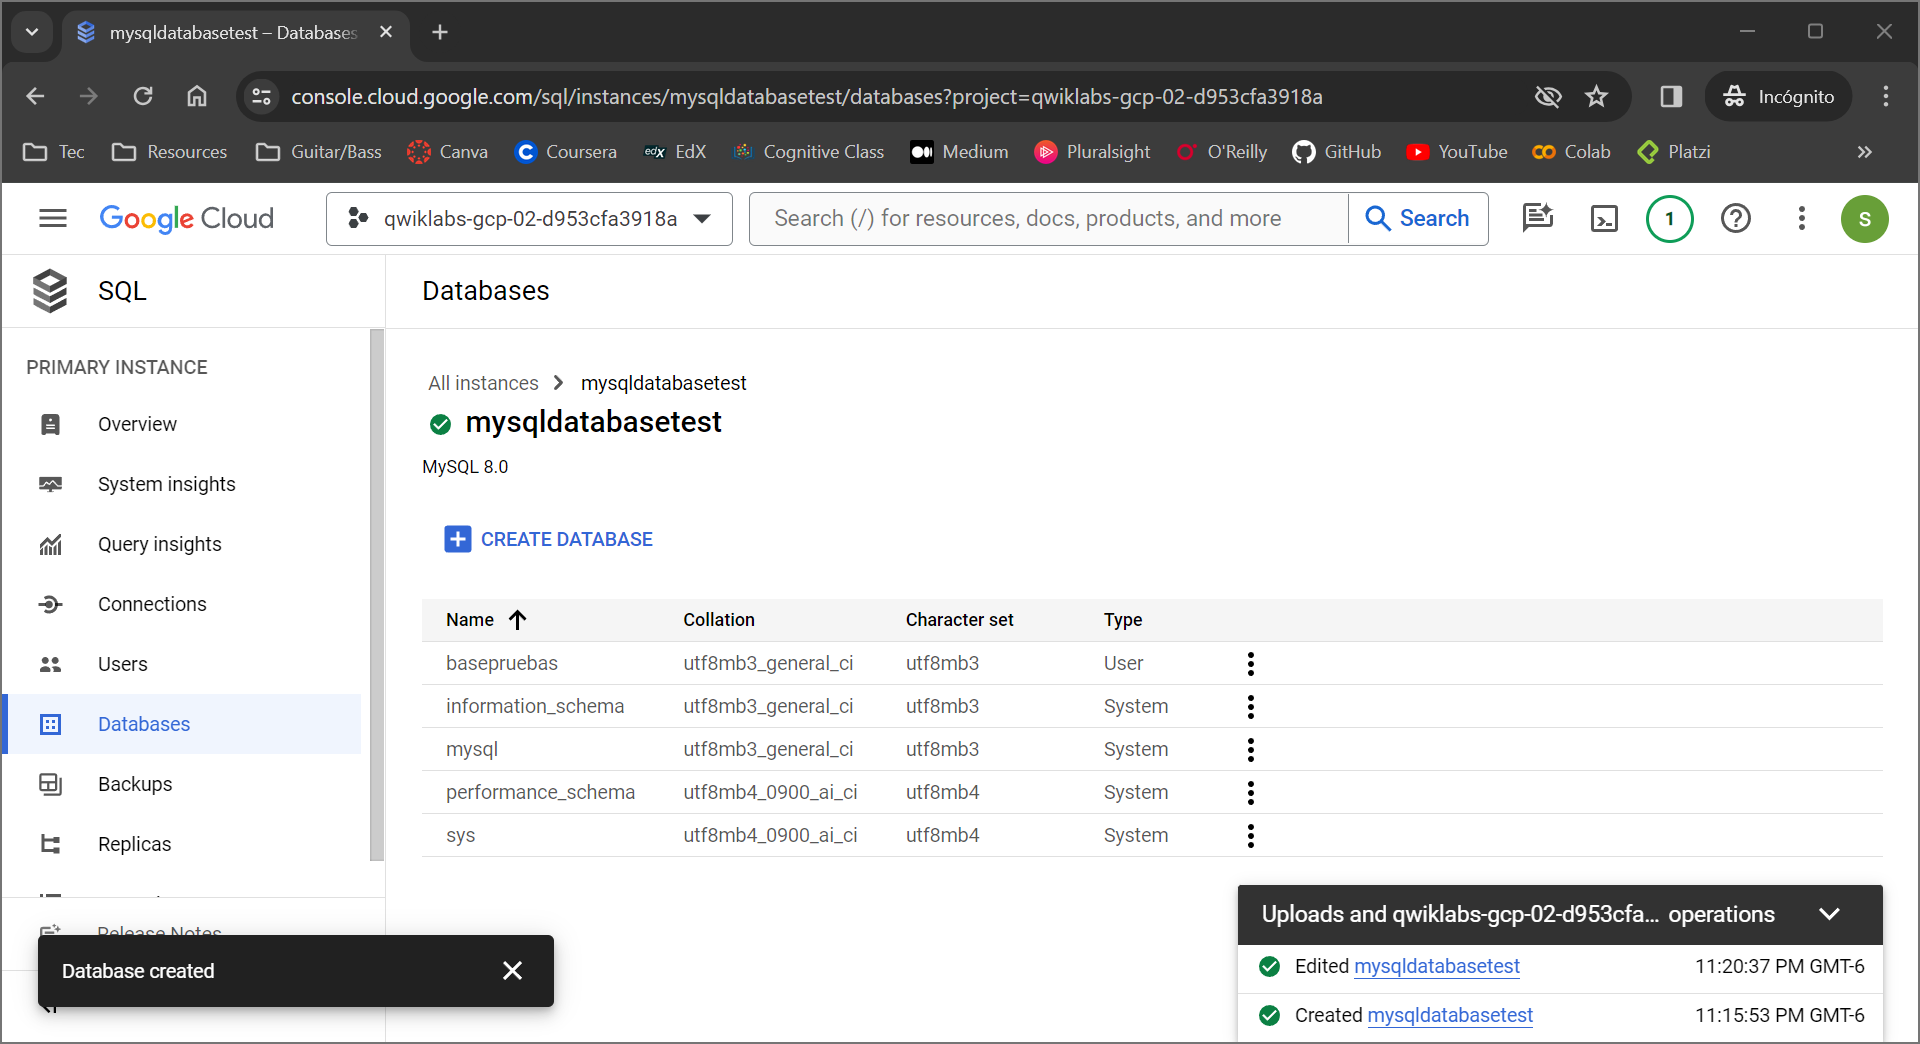
\includegraphics[width=.7\linewidth]{M4_Servicios_Cómputo_en_la_Nube/Tarea_6_Creación_sistema_administración_Base_de_Datos/reporte/figuras/2_2_2_Google_DBMS.png}
    \captionof{lstlisting}{Creación de la base de datos en Google}
    \label{fig:2_2_2_Google_DBMS}
\end{figure}

Posteriormente, al igual que hicimos con la sección de Azure, a través de \textit{MySQL Workbench} establecemos la conexión con el manejador de base datos para poder modificar la base de datos previamente creada y proceder a cargar los registros nuevos.

\begin{figure}[H]
    \centering
    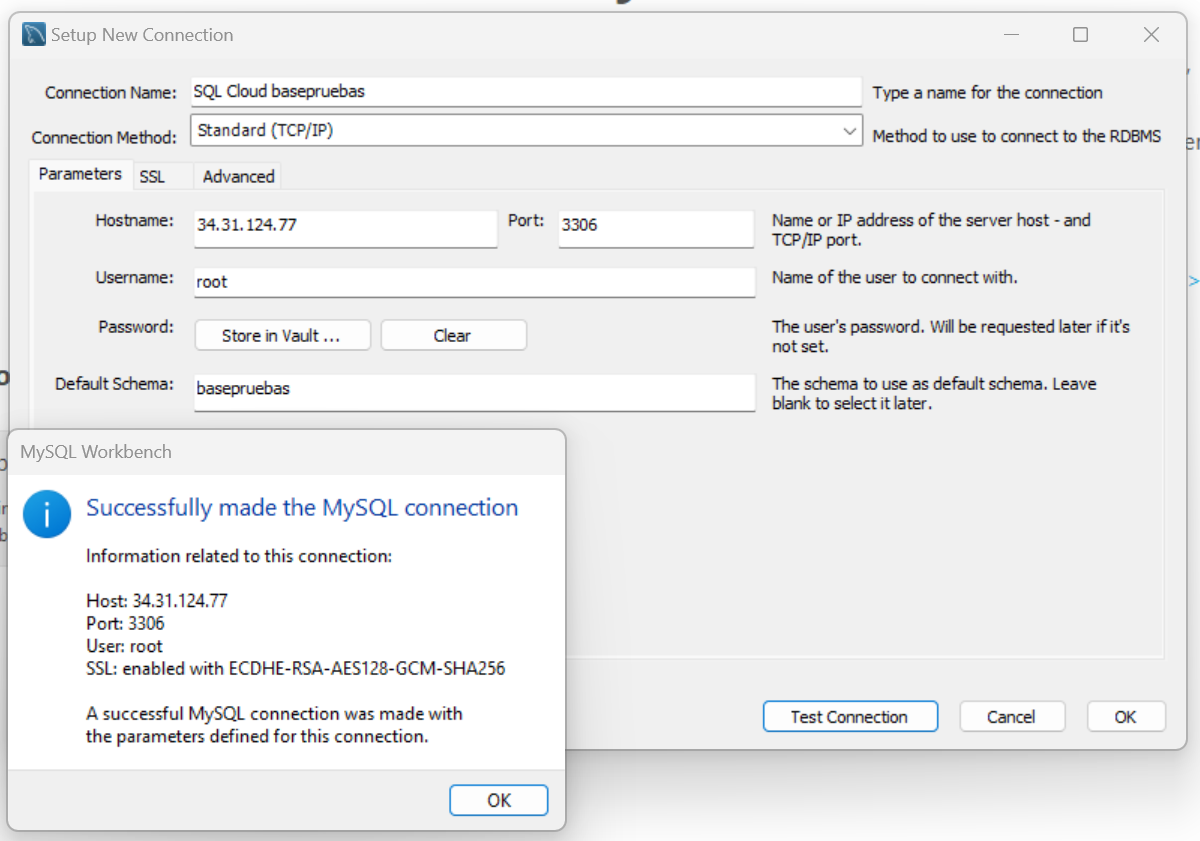
\includegraphics[width=.7\linewidth]{M4_Servicios_Cómputo_en_la_Nube/Tarea_6_Creación_sistema_administración_Base_de_Datos/reporte/figuras/2_2_3_Google_DBMS.png}
    \captionof{lstlisting}{Estableciendo conexión con el BSDM de Google}
    \label{fig:2_2_3_Google_DBMS}
\end{figure}


\subsection{Carga de los registros nuevos}

En \textit{mySQL} accedemos a la nueva base datos que creamos a través de la opción de \textit{schemas} para poder ver la base de datos y sus componentes como tablas y vistas. Posteriormente creamos una tabla con una estructura como se ve en la figura \ref{fig:2_3_1_Google_DBMS} para poder alojar la información la cual será una base de datos que representa la información ficticia de alumnos.

\begin{figure}[H]
    \centering
    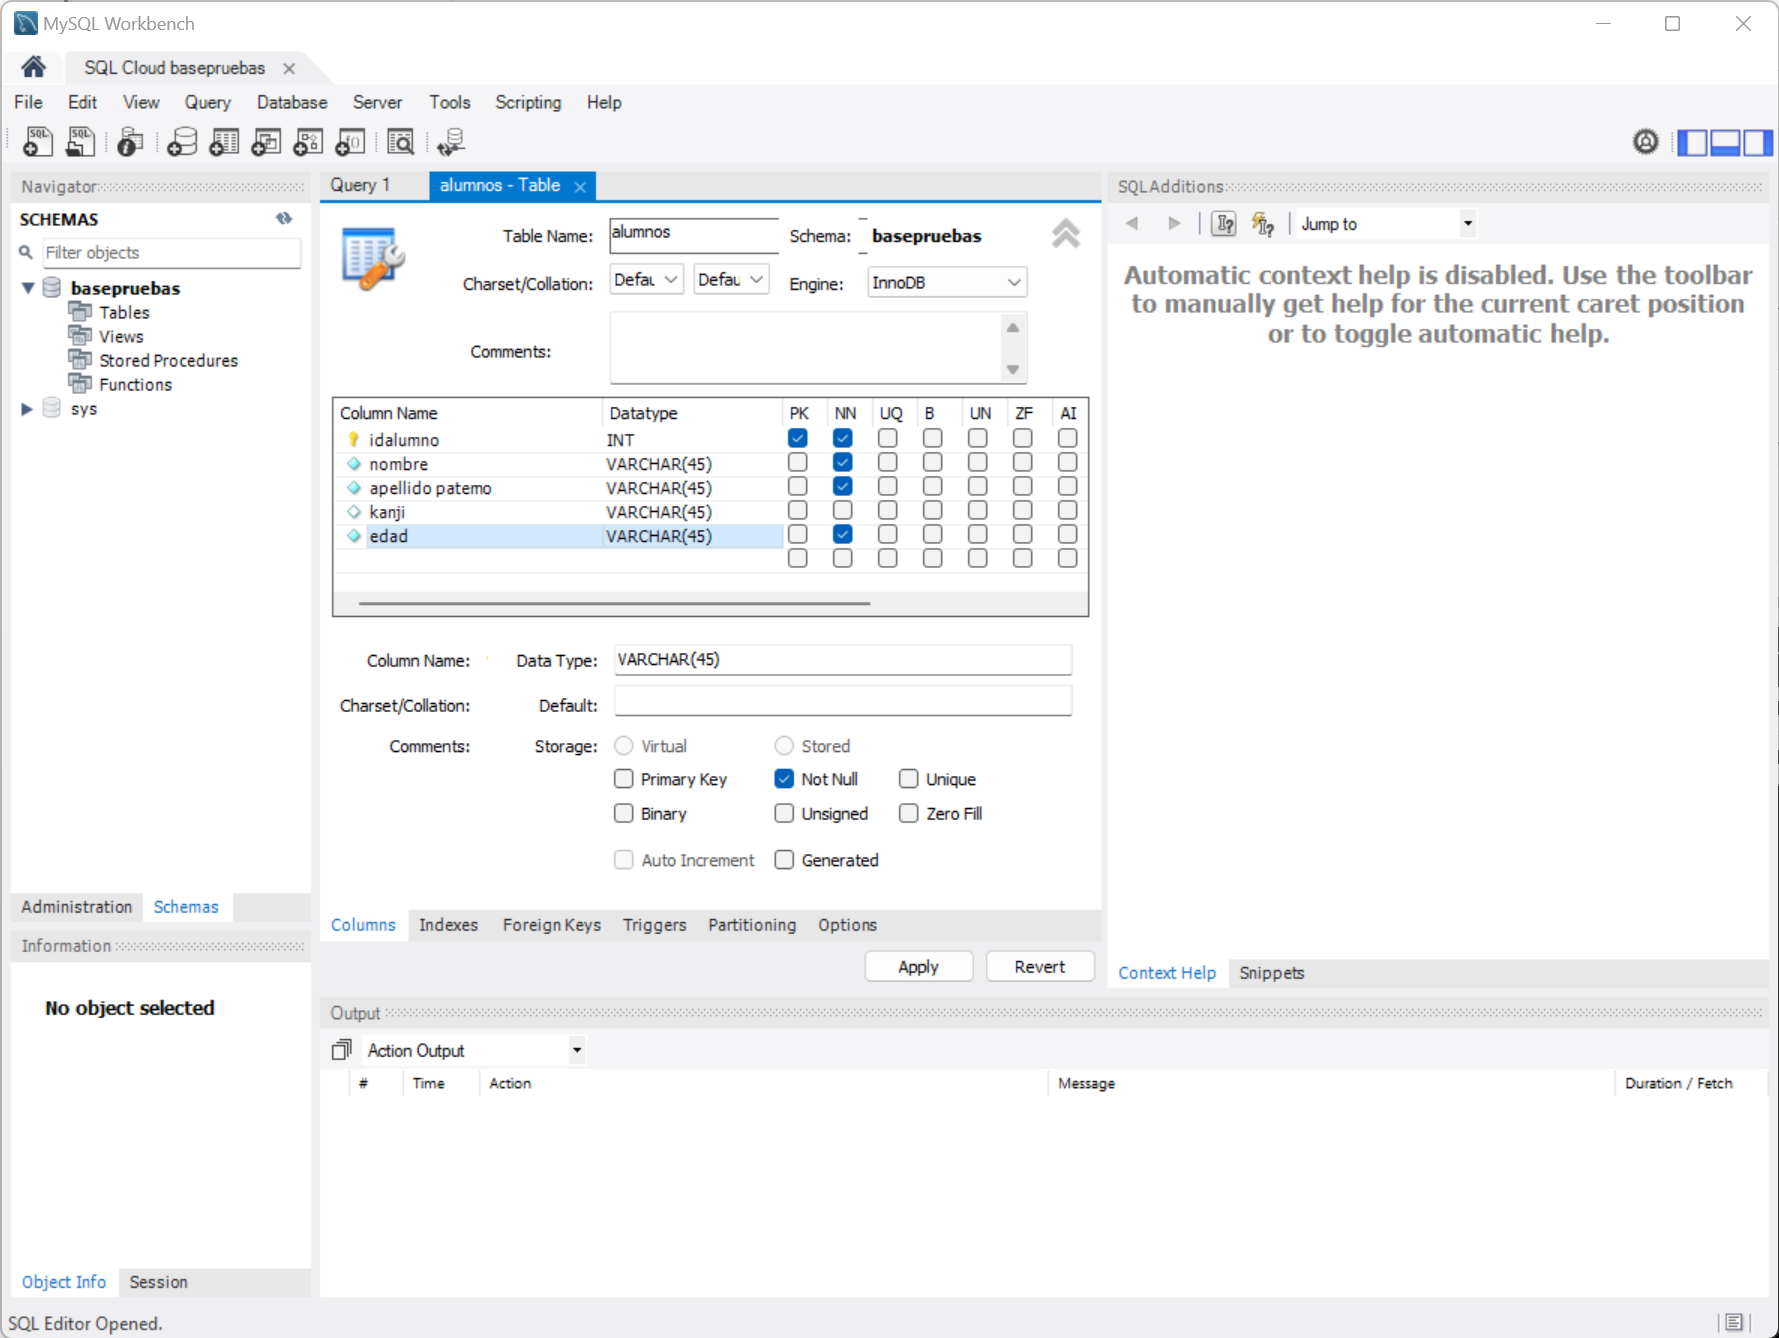
\includegraphics[width=.65\linewidth]{M4_Servicios_Cómputo_en_la_Nube/Tarea_6_Creación_sistema_administración_Base_de_Datos/reporte/figuras/2_3_1_Google_DBMS.png}
    \captionof{lstlisting}{Carga de los nuevos registros de la Base de Datos de MySQL}
    \label{fig:2_3_1_Google_DBMS}
\end{figure}

En la figura \ref{fig:2_3_2_Google_DBMS} podemos observar las sentencias que SQL estará mandando a nuestro manejador de Base de Datos en la Nube.

\begin{figure}[H]
    \centering
    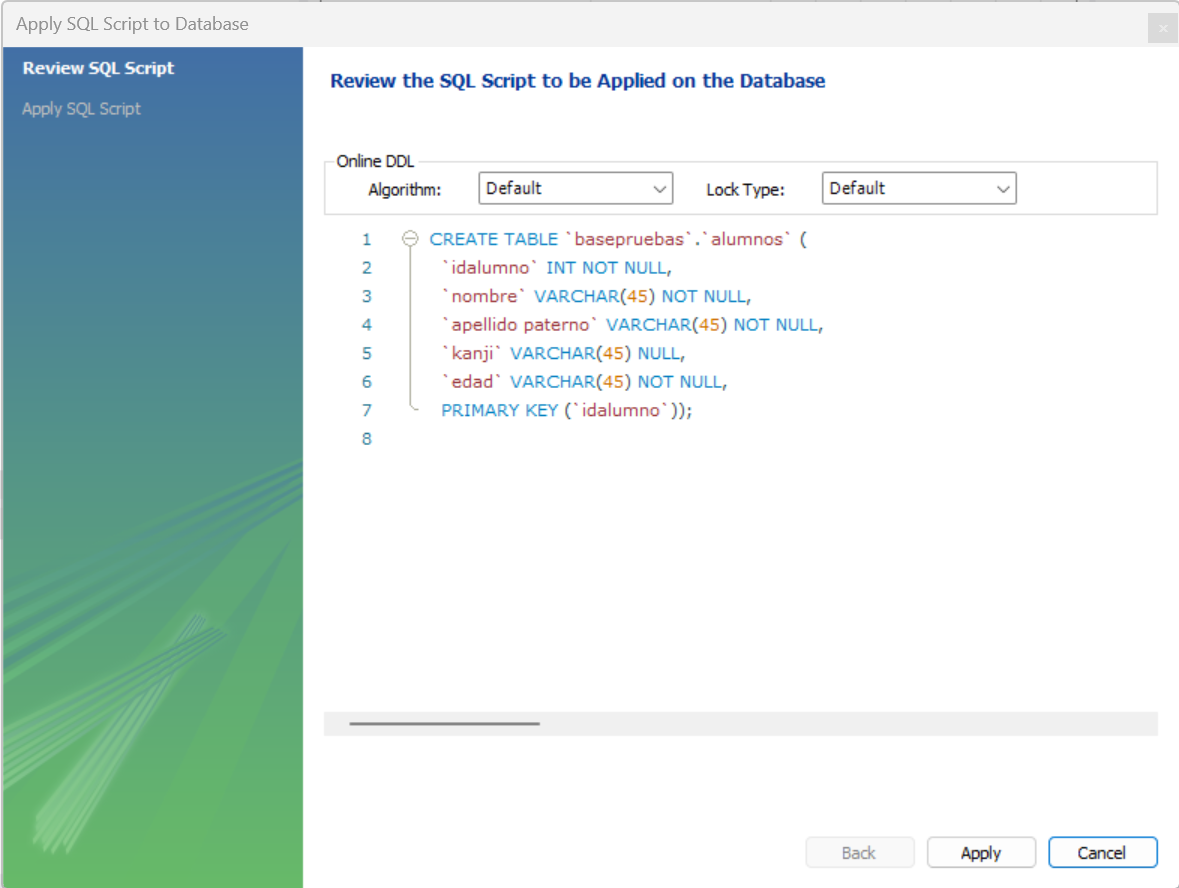
\includegraphics[width=.65\linewidth]{M4_Servicios_Cómputo_en_la_Nube/Tarea_6_Creación_sistema_administración_Base_de_Datos/reporte/figuras/2_3_2_Google_DBMS.png}
    \captionof{lstlisting}{Carga de los nuevos registros de la Base de Datos de MySQL}
    \label{fig:2_3_2_Google_DBMS}
\end{figure}

Finalmente, populamos la tabla de alumnos con algunos valores ficticios y al momento de mandar los datos a la nube observamos como los datos ingresados tienen un \textbf{id} el cual es asignado por el manejador como se observa en la figura \ref{fig:2_3_3_Google_DBMS}, de esta manera podemos corroborar que los datos ya se encuentran en la nube.

\begin{figure}[H]
    \centering
    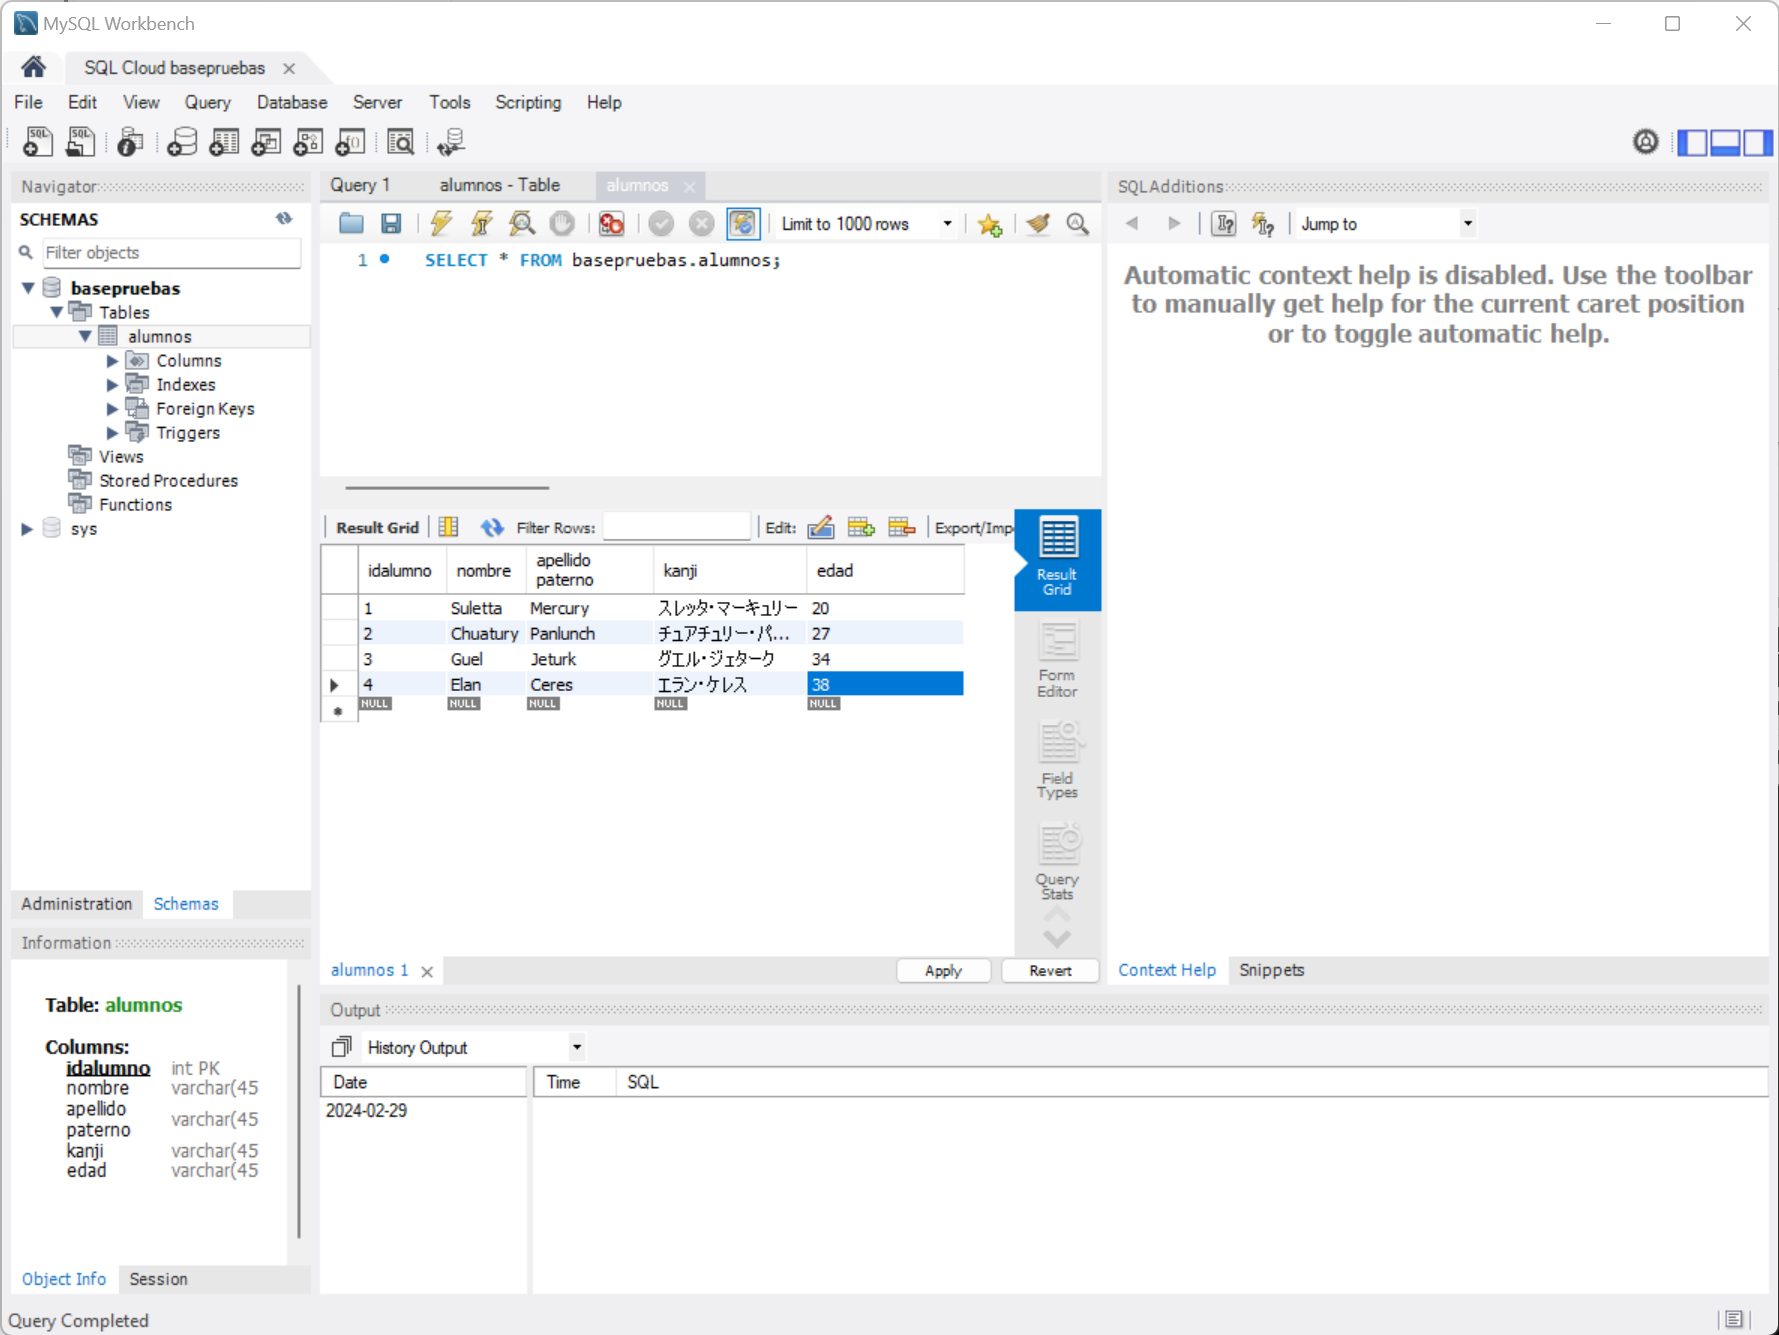
\includegraphics[width=.65\linewidth]{M4_Servicios_Cómputo_en_la_Nube/Tarea_6_Creación_sistema_administración_Base_de_Datos/reporte/figuras/2_3_3_Google_DBMS.png}
    \captionof{lstlisting}{Carga de los nuevos registros de la Base de Datos de MySQL}
    \label{fig:2_3_3_Google_DBMS}
\end{figure}


\section{Reflexión de los DataBase Management System (DBMS) en la Nube}

En la actividad realizada pudimos experimentar la creación de un sistema de manejador de bases de datos utilizando Microsoft Azure y Google Cloud con los cuales pudimos crear una base de datos MySQL que pudimos modificar y actualizar en la nube. El proceso fue muy sencillo e intuitivo con lo cual pudimos darnos cuenta que utilizar servicios de la nube es ideal para bases de datos estructuradas e incluso también para aquellas que no son estructuradas. 

\vspace{.5em}

A comparación de cuando realizamos el ejercicio de Máquinas Virtuales, en este caso se nos hizo más sencillo la realización del DBMS con Google e incluso notamos que fue menos tardado. De igual manera algo que nos llama la atención es que en Azure recibimos más alertas sobre el tipo de conexión a través de una URL publica como lo realizamos. 

\vspace{.5em}

Algo que nos hubiera gustado hacer con Azure es ver como poder visualizar la base de datos que cargamos con algún visualizador como PowerBI, será algo que más adelante estaremos explorando y para poder de igual manera aprovechar el potencial que tiene el cómputo en la nube y el poder tener soluciones integradas, por ejemplo, de almacenamiento de bases de datos y de visualización de las mismas.

\end{document}